%%%%%%%%%%%%%%%%%%%%%%%%%%%%%%%%%%%%%%%%%%%%%%%%%%%%%%%%%%%%%%%%%%%%%%%%%%%%%%%%%
%
%  Studienarbeit Vorname Name Datum         
%  "Titel"
%  Lehrstuhl fuer Mustererkennung, FAU Erlangen-Nuernberg
%
%%%%%%%%%%%%%%%%%%%%%%%%%%%%%%%%%%%%%%%%%%%%%%%%%%%%%%%%%%%%%%%%%%%%%%%%%%%%%%%%%

% ++ LME LateX Dokument 
%    Die Verwendung der option "german" bindet german.sty ein.
%    For english papers, use the "english" option and talk to your advisor.
%\documentclass[german,bt]{lmedoc}
\documentclass[english,bt]{lmedoc}
\bibliographystyle{wmaainf}


% ++ Umlaut Unterstuetzung
%    Paket "inputenc" kann verwendet werden, um z.B. Umlaute oder das scharfe S
%    direkt (als Nicht-ASCII-Zeichen) einzubinden. Dabei auf die korrekte
%    Kodiermethode achten (z.B. Linux: latin1)! 
%\usepackage[latin1]{inputenc}
\usepackage{amssymb}
\usepackage{graphicx}
\usepackage{graphics}
\usepackage[T1]{fontenc}
\usepackage{float}
\usepackage[hang,nooneline]{subfigure}
\usepackage{algorithm}
\usepackage{algpseudocode}

\usepackage{selinput}
\SelectInputMappings{
  adieresis={�},
  germandbls={�},
  Euro={�}
}
\usepackage[pdftex,colorlinks=false,linkcolor=darkblue,pdfpagelayout=TwoPageRight,pdftitle={Determining the Camera Response Function},pdfauthor={Dominik Neumann}]{hyperref}



 
\def\sectionautorefname{Section}             % I want to have capital first letter for autoref section!
\def\subsectionautorefname{Subsection}       % I want to have capital first letter for autoref subsection!
\def\subsubsectionautorefname{Subsubsection} % I want to have capital first letter for autoref subsubsection!
\def\chapterautorefname{Chapter}             % I want to have capital first letter for autoref section!
\def\subfigureautorefname{\figureautorefname} 	% Figure name also with subfloats
\newcommand{\algorithmautorefname}{Algorithm}
\newcommand{\theHalgorithm}{\arabic{algorithm}}



% ++ es werden keine underfull hboxes als Fehler ausgegeben,
%    da das ja nur hei�t, dass die Seite noch nicht ganz voll ist
\hbadness=10000


\includeonly{bt01, bt02, bt03, bt04, bt05, bt06, bt07, bt08, bt09, bt10, bt11, bt-lit, bt-lof, bt-lot}

\pagenumbering{roman}

\begin{document}
\clearpage
  \begin{deckblatt}
    \Titel{Determining the Camera Response Function}
    \Name{Neumann}
    \Vorname{Dominik}
    \Geburtsort{Amberg}
    \Geburtsdatum{August $\text{8}^\text{th}$, 1987}
    \Betreuer{Dipl.-Inf. Christian Riess, Dr. Elli Angelopoulou}
    \Start{March $\text{1}^\text{st}$, 2010}
    \Ende{August $\text{11}^\text{th}$, 2010}
  \end{deckblatt}


\cleardoublepage


Ich versichere, dass ich die Arbeit ohne fremde Hilfe und ohne Benutzung
anderer als der angegebenen Quellen angefertigt habe und dass die Arbeit
in gleicher oder "ahnlicher Form noch keiner anderen Pr"ufungsbeh"orde
vorgelegen hat und von dieser als Teil einer Pr"ufungsleistung
angenommen wurde. Alle Ausf"uhrungen, die w"ortlich oder sinngem"a"s
"ubernommen wurden, sind als solche gekennzeichnet.
\\

Die Richtlinien des Lehrstuhls f"ur Studien- und Diplomarbeiten
habe ich gelesen und anerkannt, insbesondere die Regelung des
Nutzungsrechts. \\[15mm]
Erlangen, den 11. August 2010 \hspace{6.0cm} \\[10mm]

\clearpage

\begin{center}
\bfseries
Acknowledgments
\normalfont
\end{center}
%
Thank you to everyone who has supported me in creating this thesis. Especially to my advisor Christian Riess for the selfless support and his great efforts to explain things clearly and simply. Special thanks also to Isabella Haidl, Felix Lugauer and the people from ``Bildlabor'', Eva Eibenberger, Johannes Jordan, Elli Angelopoulou and to my family.

\cleardoublepage


\bfseries
\begin{center}
"Ubersicht
\end{center}
\normalfont
Heutige Digitalkameras �ndern die gemessenen Daten nichtlinear ab, damit optisch ansprechendere Bilder entstehen. All diese nichtlinearen Ver"anderungen lassen sich zu einer einzigen Funktion zusammenfassen, der Camera Response Function (CRF). Einige Algorithmen aus dem Bereich des Rechnersehens ben"otigen allerdings Bilder, deren Intensit"atswerte m"oglichst linear zu der am Sensor gemessenen Beleuchtungsst"arke sind. In letzter Zeit wurden einige Ans"atze vorgestellt, die sich damit befassen, die CRF einer Kamera zu sch"atzen (und zu invertieren). Die meisten funktionieren allerdings nicht auf beliebigen Bildern, da sie als Eingabe auf mehrere Bilder von der selben Kamera unter bestimmten Aufnahmebedingungen angewiesen sind.

Es werden zwei Ans"atze vorgestellt, die die CRF aus einem einzelnen Bild sch"atzen k"onnen. Der erste Ansatz basiert auf physikalischen Eigenschaften. Trotz sorgf"altigen Studiums konnten wir bei dieser Methode keine zufriedenstellenden Resultate erzielen. Jedoch schlagen wir einen Ansatz f"ur weitere Untersuchungen vor. Die zweite Methode baut auf maschinellem Lernen auf und lieferte gute Ergebnisse. Die Evaluation erfolgte mittels verschiedener Tests, darunter ein Stabilit"atstest. Die gesch"atzten CRFs von Bildern der selben Kamera wurden auf "Ahnlichkeit hin untersucht. Die Robustheit der Methode h"angt sehr stark von der Wahl von drei Parametern ab. Es hat sich gezeigt, dass die Ergebnisse erheblich verbessert werden k"onnen, wenn zus"atzliches Wissen "uber die Art der CRF oder die Qualit"at der Daten zur Verf"ugung steht.




\bfseries
\begin{center}
Abstract
\end{center}
\normalfont
Typical digital cameras usually add nonlinearities to the sensed data to make the image look more visually pleasing. These nonlinearities can be summarized as a single function, the camera response function (CRF).  However, many computer vision algorithms require images, where the intensities are approximately linearly related to scene radiance. Recently, several approaches to estimate (and invert) the CRF of a camera were proposed. Most of them require several images taken in constrained environments. Such methods can not be applied on arbitrary images. 

In this thesis, two approaches are presented, which are explicitly designed to work on a single image. First, we followed a physics-based approach. Despite thorough studies, we could not achieve satisfying results. Nevertheless, an approach for further examination of this method is proposed. Second, we implemented a machine learning-based approach, which provided good results. A variety of tests was applied to evaluate it, including stability tests. For the same camera, the similarity of CRF estimates on different images is examined. The robustness is heavily dependent on the choice of three parameters. It turned out, that the results can be significantly improved by additional knowledge on the type of CRF in the camera and the quality of the data.



\cleardoublepage

\tableofcontents

\cleardoublepage \pagenumbering{arabic}

\chapter{Introduction}
\label{chap:introduction}

\section{Motivation}
\label{sec:motivation}
Have you ever wondered, why your images taken by your digital camera sometimes look even better than the reality? There is no magic, it starts with inevitable physics and is afterwards mainly controlled by the camera manufacturers by constructing microchips, which process the acquired images in a way such that they appear much more visually pleasing. But sometimes, this enforced beauty is also a curse.

Many computer vision algorithms rely on the assumption, that the input images have a linear relationship to the real-world scene radiance recorded at the camera sensor. For instance, on a very low level, the latter is needed for an accurate comparison of images from two different digital cameras. Another example for more complex analysis is to use the brightness values in digital images as physical measures.

One of these applications using the latter is the estimation of the illuminant color as done in \cite{tancolorconstancy}, which on the other hand has significant impact on a variety of computer vision problems like \emph{Color Constancy} \cite{finlayson2001color} or the related \emph{Color Constant Color Indexing} \cite{funt1995color} for the retrieval of images from databases. Another frequently used application is the construction of high dynamic range (HDR) images without having a special purpose camera. Techniques are proposed in \cite{mann1995being, CAVE_0068} and \cite{debevec2008recovering}. \emph{Photometric Stereo} methods \cite{woodham1980photometric, basri2007photometric} recover the shape and reflectance properties of an object using multiple images with varying lighting conditions, but a fixed viewpoint. \emph{Shape from Shading} \cite{zhang1999shape} is some kind of a special case for the latter, where the observation is just a single image. A result from such an algorithm is shown in \autoref{fig:shapefromshading}.

\begin{figure}
	\centering
	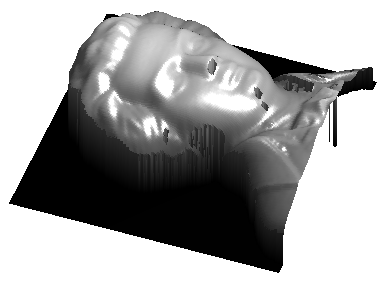
\includegraphics[width=0.3\textwidth]{images/shapefromshading.png}
	\caption[Example result of \emph{Shape from Shading}]{Example result of \emph{Shape from Shading}. Picture courtesy of R. Zhang.}
	\label{fig:shapefromshading}
\end{figure}

However, due to nonlinear camera response functions (CRF), for most digital cameras, this assumption does not hold, \hbox{i.e.} the linearity is not maintained in the observed image. Therefore, the \emph{relinearization} of the measured image intensity is very important for the above mentioned and many other algorithms to work properly. To do so, the particular CRF must be estimated and inverted. This inverted CRF can be applied to the measured image intensities to obtain an image approximately linear to the real-world scene radiance.





\section{Related Work}
\label{sec:relatedwork}
There is a huge literature on the estimation of camera response functions. Primarily it can be separated into techniques requiring special equipment, methods using several images of the same scene with known but varying camera settings and on the other hand approaches, which only need very limited information, trying to estimate the CRF from only a single intensity image. The latter are the only methods which can both operate under laboratory conditions, \hbox{i.e.} possessing the examined camera and possibly some equipment, but also when just the image and no additional knowledge is available. For instance, this is the case if the examination of camera responses from images downloaded from online resources like \emph{picasaweb} or \emph{flickr} is targeted. The two methods implemented during the creation of this thesis can both operate on single images.

The probably most popular example, where special equipment is required, is the estimation using a color chart of known reflectances like a Macbeth chart \cite{chang1996rgb}. This chart includes a set of patches in different shades of gray, starting from white and ending up in black, as well as other precisely defined colors, all in all 26 distinctive patches. These can be used to obtain some discrete samples of the actual CRF. The biggest problem here is to ensure uniform lighting.

One approach is to use a high quality light source inside a large dark room. The light source should be as far away from the chart as possible. Another approach is to place the chart outdoors under direct illumination. Note that the results will differ under these two conditions, because the illumination color will be different. 

\begin{figure}[htbp]
  \centering
  \subfigure[shortest period]{
    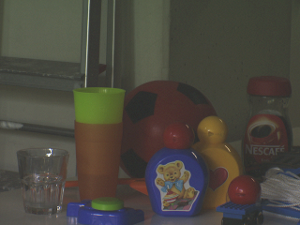
\includegraphics[width=0.22\textwidth]{images/exposure0.png} 
  }
  \subfigure[short period]{
    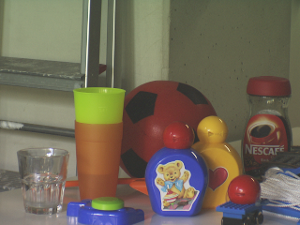
\includegraphics[width=0.22\textwidth]{images/exposure1.png} 
  }
  \subfigure[long period]{
    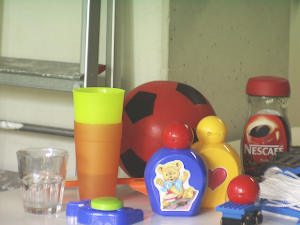
\includegraphics[width=0.22\textwidth]{images/exposure2.png} 
  }
  \subfigure[longest period]{
    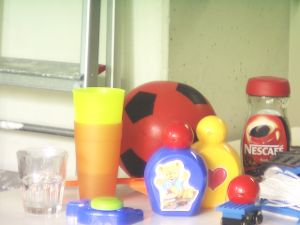
\includegraphics[width=0.22\textwidth]{images/exposure3.png} 
  }
  \caption[Estimating CRF by changing exposure settings]{Estimating CRF through changing exposure settings. Multiple same-scene images with varying exposure periods are required.}
  \label{fig:multipleexposures}
\end{figure}

Due to the fact that the camera response is a continuous function, some kind of interpolation incorporating these sampling points is applied. In theory, the effects of this interpolation have also to be inverted. Nevertheless, this manual technique provides ground-truth values. Hence, it is utilized for measuring fitting scores of different CRF approximation models, for instance the empirical model of response (EMoR) presented in \cite{CAVE_0091}, the polynomial model from \cite{CAVE_0068}, gamma curves as used in \cite{mann1995being} and \cite{farid2001aa} or the generalized gamma curve model from \cite{ng_cvpr07} presented in \autoref{subsubsec:ggcm} of this thesis.

S. K. Nayar and T. Mitsunaga presented the ``Radiometric Self Calibration'' in 1999 \cite{CAVE_0068}. This algorithm requires a set of images of an arbitrary scene, captured with several different exposure settings (for an illustration see \autoref{fig:multipleexposures}). For each image, different shutter speed configurations and different aperture settings are used. The primarily intended application for this method is the automatic generation of accurate high dynamic range images. A demonstration is available on their website\footnote{\url{http://www.cs.columbia.edu/CAVE/software/rascal/rrhome.php}}.

Another CRF estimation approach introduced by the same authors was published one year later, titled ``High Dynamic Range Imaging: Spatially Varying Pixel Exposures'' \cite{nayar2000high}. Here, they utilize an optical filter with spatially varying transmittance and they show that this variation has a certain correspondence to the irradiance ratio. This information is used to estimate the CRF from a single image and thus their approach -- unlike the one published one year earlier -- does not require to capture a whole set of images of a static scene using separate camera settings.

A more recent method published in 2008 \cite{takamatsu2008estimatingECCV} requires several static same-scene images, but without varying the camera settings. J. Takamatsu, Y. Matsushita and K. Ikeuchi use a so-called \emph{Probabilistic Intensity Similarity Measure} (PISM), which represents the likelihood of two intensity observations corresponding to the same scene radiance. Due to the presence of noise, having two or more images of the same scene, these observations will slightly differ. They show that the PSIM is strongly related to the particular CRF and thus maximizing this intensity similarity function for all pixels over a set of same-scene images leads to a reliable estimation of the camera response. Unlike other methods, this one is independent of any particular statistical prior models. Real-world experiments demonstrate the effectiveness of this method for digital cameras as well as video cameras.

In ``Blind Inverse Gamma Correction'' \cite{farid2001aa}, H. Farid measures the effects of the gamma correction from a single image without any knowledge of the used camera or any calibration information. It is shown on both, natural and synthetic images, that the error between the estimated and the ground-truth gamma curve is in most cases very small. But the problem here is, that for almost every real-world camera, the camera response is a combined effect of various internal operations, not only gamma correction. Hence, this method does not really fit to the approach of estimating a complete CRF.





\section{Patents}
\label{sec:patents}
There are two relevant patents related to publications by S. Lin et \hbox{al.} US patent 7450754 from November 2008 is entirely based on \cite{Lin04radiometriccalibration} and thus the claimed method requires three channel RGB images for estimating the CRF. Due to this method being part of this thesis, it is described in detail in \autoref{sec:radcal}. The application number is 10/809167, filed in March 2004. The 2005 filed (application number 11/156988) US patent 7463769 issued in December 2008 claims another approach, ``Determining the Radiometric Response Function from a Single Grayscale Image'' \cite{lin2005determining}, which uses a statistical feature of graylevel histograms at edge regions to gain information for radiometric calibration. This method is -- as its name implies -- intended for grayscale images, but can also be used for images with more than one channel by analyzing each channel separately. The approach can be seen as a grayscale pendant to \cite{Lin04radiometriccalibration}. Hence for both, color and grayscale images, their methods are covered by US patents.

Another related US patent numbered 7505606 from March 2009, filed on May 2005, is titled ``Detecting Doctored Images using Camera Response Normality and Consistency'', where parts of the method proposed in the identically named publication \cite{rongrong-detecting} are claimed. Sets of patches of an image containing cues on the applied CRF are obtained. A support vector machine (SVM) is trained with some features extracted from examples of normal and abnormal inverse CRFs to be able to classify given inverse CRFs into normal and abnormal ones. This method helps distinguishing natural and tampered images. Although the recovery of inverse CRFs from images to map the intensities back to irradiance is mentioned in their list of claims, it is not presented in detail. Some figures shown in the drawings part are very similar to those in a publication of an approach presented in this thesis \cite{Lin04radiometriccalibration}, but the claims are mainly on training the SVM and classifying sets of patches for image forensics. So this patent does not severely limit implementations of CRF estimation.

All three patents above are assigned to \emph{Microsoft Corporation}, Redmond, WA (US).



\section{Thesis Overview}
\label{sec:overview}
In \autoref{chap:crf}, an overview of the camera-internal processes is given. The first step, the measuring of scene radiance is presented in \autoref{sec:radiancetoirradiance} and the second step, the transformation from image irradiance to image intensity in \autoref{sec:irradiancetointensity}. Afterwards, in \autoref{chap:description} the two methods treated in this work are described, starting with \cite{Lin04radiometriccalibration} in \autoref{sec:radcal}. The second method \cite{ng_cvpr07} is described in \autoref{sec:geoinv}. In \autoref{chap:evaluation}, at first, a short overview of the problems we encountered when implementing the second method is given in \autoref{sec:challenges}. The actual evaluation is about the first approach and starts with the examination of the capabilities of the data acquisition step in \autoref{sec:capabilitiesofdataacqu} by varying two crucial parameters. Tests with synthetic data in \autoref{sec:syntheticdata} demonstrate the influence of the parameter $\lambda$. In \autoref{sec:stability} the robustness of the method is examined by utilizing sets of same-camera images. Finally, in \autoref{chap:summaryoutlook}, a short summary and outlook are given.   % Einfuehrung (\chapter{Einf"uhrung})
\cleardoublepage
\chapter{The Camera Response}
\label{chap:crf}
In the following paragraph, the essential terminology for this thesis is introduced in combination with a short overview. In \autoref{fig:crfoverview}, a visualized overview is given.

\emph{Scene radiance} is the composition of the real-world radiances in the natural scene, \hbox{i.e.} the amount of light. Note that scene radiance is only dependent on the physics of the scene. It is not yet affected by any technically induced disturbances. Then scene radiance is transformed to \emph{image irradiance} through measuring discrete intensity values on a light-sensitive sensor array, most commonly a CCD chip for digital cameras. With some special cameras designed for scientific purposes, it is now possible to extract such RAW images. But most commonly, the output of a digital camera -- after the post-processing of the image irradiance by a camera-internal processor -- is \emph{image intensity}.
In this work, the focus is on the determination of major changes between two consecutive in-camera transformations.

\begin{figure}[p]
	\centering
	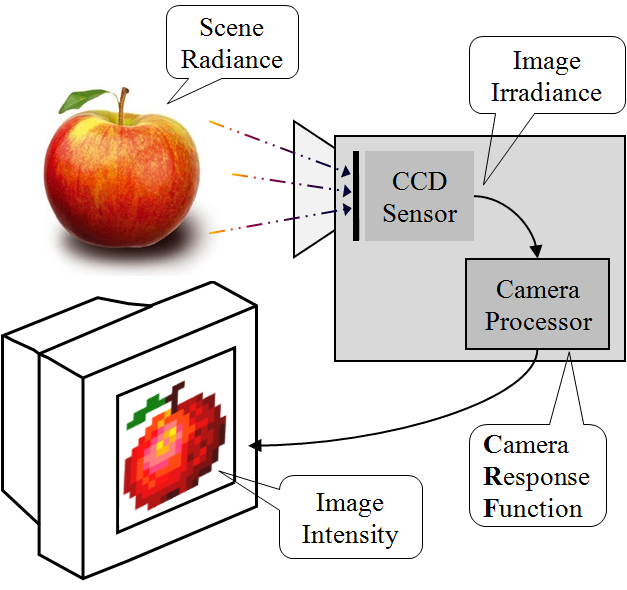
\includegraphics[width=0.8\textwidth]{images/crf_overview.png}
	\caption[On the overview terminology]{On the overview terminology. The apple in the upper left illustrates a real-world scene. The grey box on the right represents a simplified digital camera, where at first light is measured through a CCD sensor and its output is afterwards post-processed by the camera-internal processor. This is where the CRF is applied. The output of the processor -- an intensity image -- is shown in the lower left (on the computer monitor).}
	\label{fig:crfoverview}
\end{figure}

\section{Measuring Scene Radiance}
\label{sec:radiancetoirradiance}
For measuring natural scene radiance, a \emph{charge-coupled device} (CCD) sensor -- invented in 1969 -- is most commonly used in consumer-quality digital cameras. Through a lens, light is projected on a photoactive array, where in each cell electric charge proportional to the amount of incoming light (photons) at that specific location is accumulated. After this so-called exposure period, the process of transferring the charge off the array begins. For each row in the array, the charge in each cell is shifted until reaching the corner cell, where the charge is converted into voltage, measured by an analog-to-digital converter and finally transferred to memory. Once all the cells in a row have been processed, the cells in the next row get measured. Although each cell and each row is measured individually, millions of cells can be sampled in a fraction of a second.

The just described functional principle of a CCD sensor measures light, not color. For that reason, digital cameras most commonly use a \emph{Bayer mask} attached to the CCD sensor to get three channel RGB information, where each $2 \times 2$ square on the CCD array has one pixel filtered red, one pixel filtered blue and two pixels filtered green (see \autoref{fig:bayermask}). The high amount of green filtered pixels is chosen due to the fact that the human eye also is much more sensitive to green than either red or blue. The filter makes the color resolution per pixel lower, but still the luminance information is collected at every pixel. The filtering causes a \emph{mosaicing} effect on the resulting CCD output, such that the final intensity image has to be reconstructed from these color CCD samples. For this purpose, \emph{demosaicing} techniques as in \cite{kimmel1998demosaicing} are available. Although better color resolution can be reached by using so-called 3CCD devices, where for each of the three colors -- red, green and blue -- a separate CCD chip is used after the light is separated by a prism, most digital cameras have a single CCD sensor built in due to significantly lower manufacturing costs.

\begin{figure}[t]
	\centering
	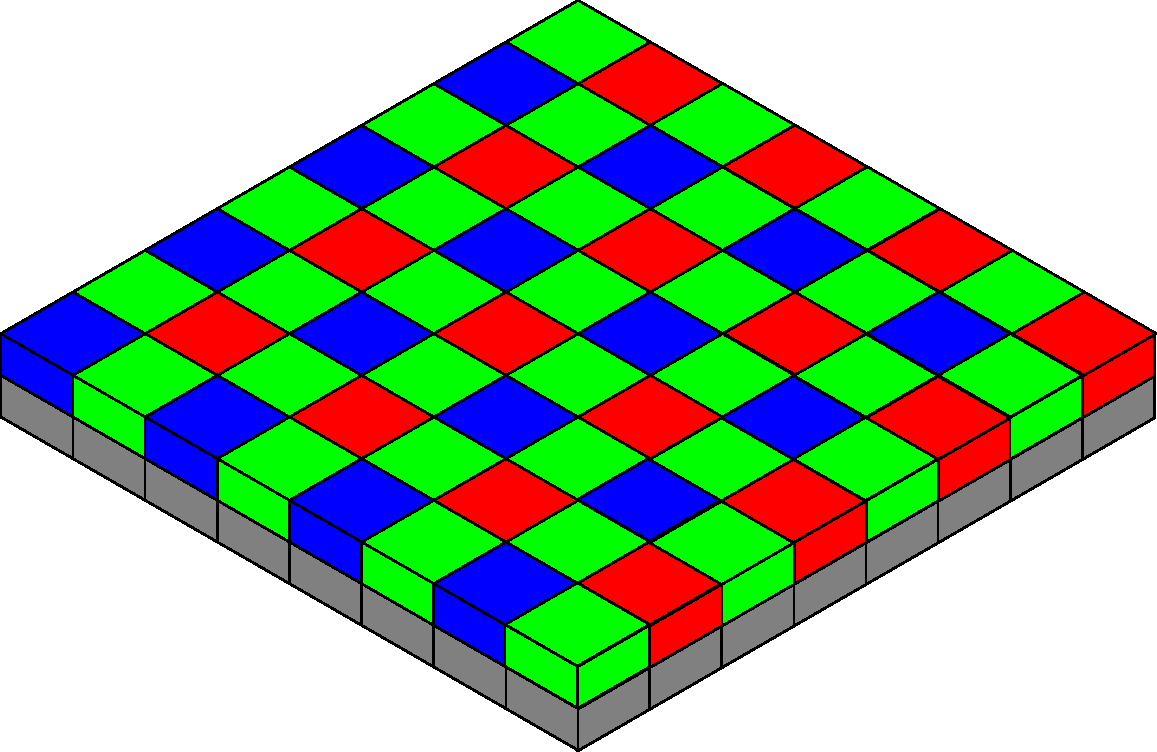
\includegraphics[width=0.5\textwidth]{images/bayerfilter.pdf}
	\caption[Bayer filter on a CCD sensor]{Bayer filter on a CCD sensor. The colored boxes sketch the Bayer mask and the underlying grey boxes the cells of the actual CCD sensor array. Note that the amount of green filtered pixels is as high as the amount of pixels for the colors red and blue combined.}
	\label{fig:bayermask}
\end{figure}

The charge in each cell is proportional to the luminance. Thus, the function, which maps scene radiance to image irradiance, is basically linear, although it may vary spatially over the image due to the presence of noise. Examining the effects caused by this transformation for going from image irradiance back to scene radiance are not part of this thesis. For further reference, confer \cite{healey1994radiometric}.


\section{Mapping Image Irradiance to Image Intensity (CRF)}
\label{sec:irradiancetointensity}
The camera response function maps image irradiance to image intensity. Having a wide range of irradiance values and just a small range of possibly measurable intensity values, nonlinearity is a simple method for compressing these values. So camera manufacturers purposefully introduce nonlinearities in the camera's electronics, \hbox{i.e.} nonlinear CRFs. A second reason is, that a few years ago, digital cameras were not yet available for the consumer market. Typically, analog cameras with photographic films were used to take photographs. So the first digital cameras aimed to mimic the properties of analog photographs, which were usually nonlinear as well. Furthermore, a variety of aesthetic effects and refinements with respect to human perception can be generated by varying the CRF, like applying gamma correction, white balancing to compensate for different light temperature or other sophisticated corrections to make the image more visually appealing.

M. Grossberg and S. Nayar examined the CRFs of 201 real-world digital cameras and video cameras as well as common brands of films. They compiled a database of real-world camera response functions (DoRF), available on their website\footnote{\url{http://www.cs.columbia.edu/CAVE/software/softlib/dorf.php}}. Their intention was to build up a solid ground-truth base for evaluating different camera response models. This database is now also used as prior knowledge for maximum a posteriori (MAP) estimations in \cite{Lin04radiometriccalibration}. All CRFs in DoRF are monotonic and normalized to $[0; 1]$.

A common assumption on CRFs is, that it is the same for each pixel in image irradiance, although in theory the CRF could vary spatially. The second assumption is that every camera response has a well defined boundary $B$, where the CRF domain goes from $B_\text{min}$ to $B_\text{max}$. Both variables can be computed easily. $B_\text{min}$ can be estimated by taking a photo with the lens cap on, $B_\text{max}$ on the other hand by photographing a very bright object such as the sun or other light sources. Parts of the image will then be saturated. Having this boundary for a camera, it is reasonable to normalize the domain to $[0; 1]$ as done in the following.
\begin{equation}
	\overline{x} = \frac{x - B_\text{min}}{B_\text{max} - B_\text{min}}, \ \ x \in B = [B_\text{min}; B_\text{max}] \enspace ,
	\label{eq:normalization}
\end{equation}
where $x$ is a measured irradiance value and $\overline{x}$ its normalization. The codomain of a CRF is also normalized, with respect to the number of available bits $\#_b$ per channel, which is usually $\#_b = 8$. So $B_\text{min} = 0$ and $B_\text{max} = 2^{\#_b}-1$ in terms of \autoref{eq:normalization}. 

The third assumption is that any CRF $f$ is strictly monotonically increasing, what makes the CRF invertible. Hence, once the CRF is determined, it can get inverted to map image intensity back to image irradiance. Some algorithms estimate this inverse function $g$ directly, which can then be transformed to $f$, if needed. All of the 201 empirically determined response curves in DoRF got transformed in a way, that these three introduced assumptions hold. Altogether, the space $W_f$ of possible CRFs and -- due to the properties of $f$ -- also the space $W_g$ of all inverse response functions are defined as
\begin{equation}
	W_\pi = \left\{\pi:\pi(0) = 0;\ \pi(1) = 1;\ \pi \ \text{strictly monotonically increasing}\right\} \enspace ,
	\label{eq:spaceofCRFs}
\end{equation}
where $\pi$ is either the CRF $f$ or the inverse CRF $g$. The normalization process is illustrated in \autoref{fig:crfnormalization}.

\begin{figure}[bth]
	\centering
	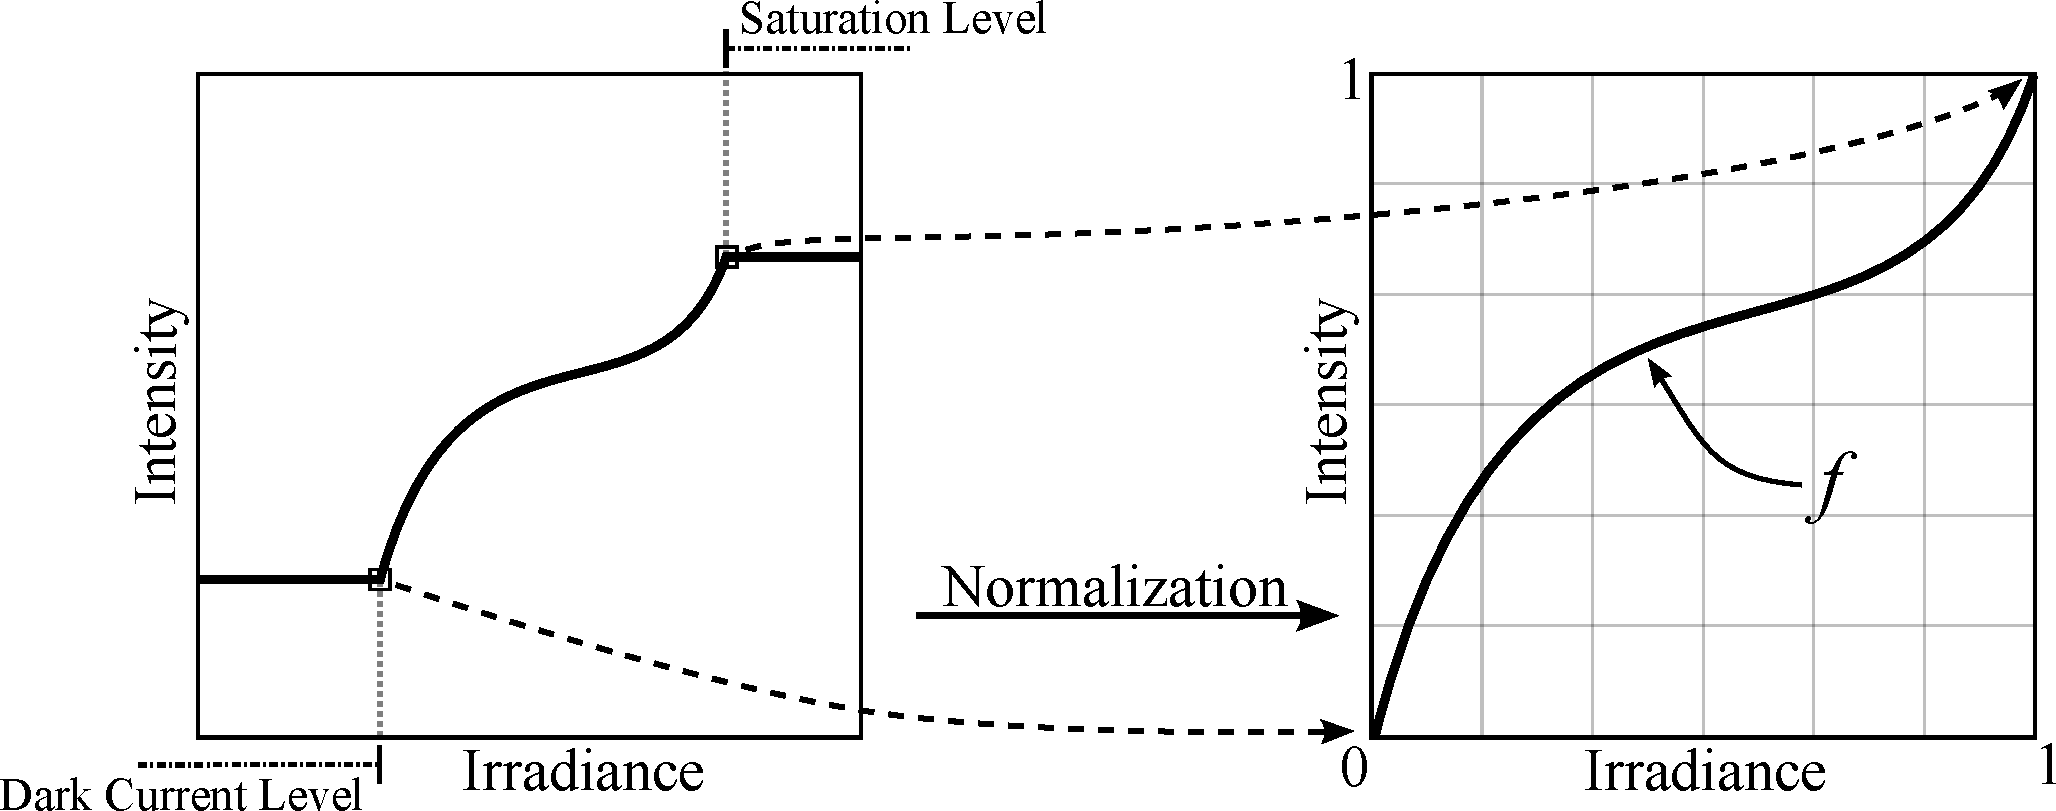
\includegraphics[width=0.8\linewidth]{images/crf_normalization.pdf}
	\caption[CRF normalization]{CRF normalization, inspired by M. Grossberg and S. Nayar. The left figure shows an example mapping from irradiance to intensity. The current levels (darkness and saturation) can not be recovered. Hence, they get cut off during the normalization process. The right figure shows the result of the normalization, a function which is called the camera response $f$. Both, domain and codomain lie within the range $[0; 1]$.}
	\label{fig:crfnormalization}
\end{figure}   % (\chapter{})
\cleardoublepage
\chapter{Description of the Methods}
\label{chap:description}
In this chapter, the two methods \cite{Lin04radiometriccalibration} and \cite{ng_cvpr07} treated in this thesis are presented. $r(x,y)$ and $R(x,y)$ are used respectively for image irradiance and image intensity, where $x$ and $y$ specify the pixel position in the coordinate frame of the image. The CRF is denoted either by $r = f(R)$ or by $R = g(r)$ in case of the inverse CRF.

Both papers share the assumptions, that the CRF of a camera is equal for \emph{every} image pixel and that the red, green and blue colors are accurately measured for each pixel (see \autoref{chap:crf}).

The implementations are written in \emph{C++} and based on the \emph{OpenCV} library \cite{opencv_library}, version 2.1 from April 2010.




\clearpage

%%%%%%%%%%%%%%%%%%%%%%
% RadCal
%%%%%%%%%%%%%%%%%%%%%%

\section{Radiometric Calibration from a Single Image}
\label{sec:radcal}
This method published by Stephen Lin et \hbox{al.} in 2004 \cite{Lin04radiometriccalibration} is among the earliest, where the automatic determination of the CRF from only a single arbitrary image is addressed. Like many other approaches from various authors, their method makes use of the 201 real world CRFs from the DoRF database compiled by M.D. Grossberg and S.K. Nayar and presented in their 2004 IEEE article \cite{CAVE_0091}.

``Radiometric Calibration from a Single Image'' requires image specific data acquisition by finding small patches in the image, which provide the data for a derivation of the applied CRF. If not sufficiently many patches are found, the method will fail either completely or lead to highly unstable estimates, because then the coverage of the $R$-space is only sparse. To overcome this, it is also possible to use more than only one image of the specific camera -- if available -- to obtain a higher amount of data.

\vspace{1cm}

\subsection{Theoretical Foundation}
\label{subsec:radcaltheory}
%This approach is based on the nonlinearity of edge color distributions.

\subsubsection{Nonlinearity of Edge Colors}
\label{subsubsec:nonlinearityofedgecolors}
Let $P$ be an image patch that contains two distinct regions separated by an edge, each having different but at most uniform colors $C_1$ and $C_2$. Due to the limited spatial resolution of a CCD sensor (visualized through the grid in \autoref{fig:illustrationedgenonlinearity}), the color of each edge pixel results in a linear combination of the two region colors $C_1$ and $C_2$. Hence, the colors of the edge pixels $C_{\text{edge}}$ lie on a line between $C_1$ and $C_2$ in RGB-space.
\begin{equation}
	C_{\text{edge}} = \alpha \cdot C_1 + (1 - \alpha) \cdot C_2 \enspace , 
	\label{eq:linearcombination}
\end{equation}
where $\alpha \in [0;1]$ denotes the ratio of the area in the pixel which is covered by $C_1$ to the total area of the pixel in scene radiance.

For an illustration of this interpolation see \autoref{fig:illustrationedgenonlinearity} on page \pageref{fig:illustrationedgenonlinearity}. The first image, \autoref{subfig:radiance}, shows an exemplary part of a scene (scene radiance) containing a clear edge and thus two regions of different color. In \autoref{subfig:radiancewitharray} the latter is overlayed by a grid, representing the discrete CCD sensor array. Note that the edge divides four of the array cells into two distinct regions each. \autoref{subfig:irradiance} shows the image irradiance after the linear interpolation inside the cells containing the edges as described in \autoref{eq:linearcombination}. The result of applying a basic CRF, a gamma curve with $\gamma = 0.4$, is presented in \autoref{subfig:intensity}.

\begin{figure}[tbp]
  \centering
  \subfigure[Radiance]{
    \label{subfig:radiance}
    
\includegraphics[width=0.22\textwidth]{images/patch.png} 
  }
  \subfigure[Radiance with grid]{
    \label{subfig:radiancewitharray}
    
\includegraphics[width=0.22\textwidth]{images/patch_with_array.png} 
  }
  \subfigure[Irradiance]{
    \label{subfig:irradiance}
    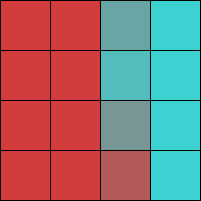
\includegraphics[width=0.22\textwidth]{images/patch_with_array_irradiance.png} 
  }
  \subfigure[Intensity]{
    \label{subfig:intensity}
    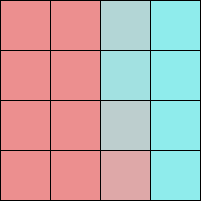
\includegraphics[width=0.22\textwidth]{images/patch_with_array_gamma04.png} 
  }
  \caption[Illustration of edge pixel distributions]{Illustration of edge pixel distributions.}
  \label{fig:illustrationedgenonlinearity}
\end{figure}

But \autoref{eq:linearcombination} only holds in the domain of \emph{image irradiance}. After the mapping from image irradiance to image intensity -- regarding the nonlinearity of the CRF -- the edge pixel colors are not located on the line between the two region colors anymore (see the plot in \autoref{fig:gammavsnogamma}). This fact is exploited to estimate the camera response function. The points on the longer one of the two lines in \autoref{fig:gammavsnogamma} depict the colors in \autoref{subfig:irradiance} and the other points the colors after the CRF transformation as in \autoref{subfig:intensity}. The lines are spanned by the region colors. This illustrates the assumption that the linear distribution changed to a nonlinear one by applying the CRF. 

\begin{figure}[bth]
	\centering
	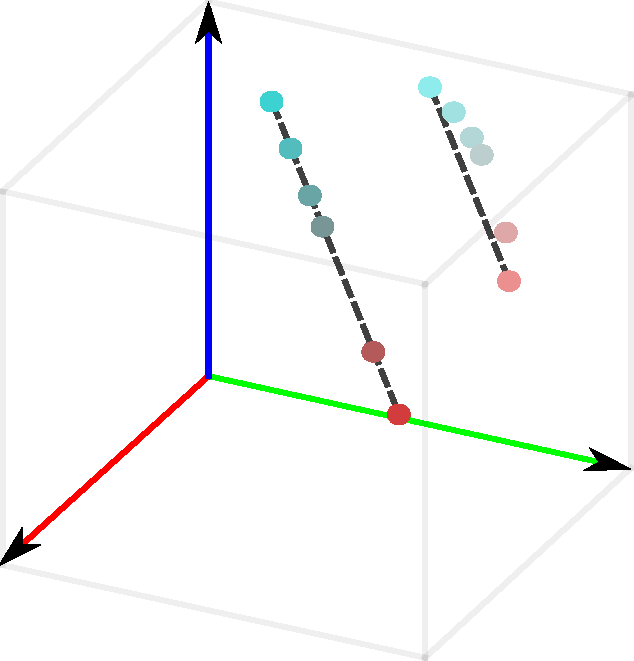
\includegraphics[width=0.4\textwidth]{plots/rgb_cube.pdf} 
  \caption[Illustration of intensity nonlinearities after gamma transformation (RGB-cube)]{Illustration of intensity nonlinearities after gamma transformation (RGB-cube).}  
  \label{fig:gammavsnogamma}
\end{figure}


\clearpage

\subsubsection{Transformation to Linear Distributions}
\label{subsubsec:transformationtolineardistributions}
Now, if a certain function $h$ can be found, which -- for every edge patch in the image -- maps the edge colors back onto the line between $h(C_1)$ and $h(C_2)$, this function is the inverse CRF $g = h$, or at least a sufficiently good approximation. Thus, for all edge patches $\omega$ in the set of edge patches $\Omega$, the distance $d(g;\omega_i)$ of the edge color $g(C_{\text{edge}})$ to the line spanned by the two region colors has to be zero:
\begin{equation}
	d(g;\omega) = \frac{\left|\left[g(C_1)-g(C_2)\right] \times \left[g(C_1)-g(C_{\text{edge}})\right] \right|} {\left|g(C_1)-g(C_2)\right|} = 0 \enspace ,
	\label{eq:distancepointtoline}
\end{equation}
where $\left|\cdot\right|$ indicates the absolute value and $\times$ denotes the cross product between two vectors. Note that the colors $C_1$, $C_2$ and $C_{\text{edge}}$ are RGB-colors and therefore three-dimensional vectors. 
The accumulated distance for all $\omega \in \Omega$ will be referred to as $D(g;\Omega) = \sum_{\omega \in \Omega}{d(g;\omega)}$ in the following. The \emph{likelihood function} $p(\Omega|g)$ is computed by an exponential distribution
\begin{equation}
	p(\Omega|g) = \frac{1}{Z} \cdot \exp({-\lambda \cdot D(g;\Omega)}) \enspace ,
	\label{eq:likelihoodfunction}
\end{equation}
where $Z$ is a normalization constant and $\lambda$ an important weighting factor, which will be examined in \autoref{chap:evaluation}.

Hence, the inverse response function and thus the CRF could be estimated by minimizing \autoref{eq:distancepointtoline}, but the accuracy can be enhanced by incorporating prior knowledge on (inverse) CRFs based on DoRF. Problems appearing when only sparse $R$-coverage is available are bypassed by using this prior knowledge. A PCA representation as presented in \cite{CAVE_0091} is chosen to model the CRFs. Additionally, $g$ can be computed straight forward
\begin{equation}
	g = g_{\text{mean}} + \vec{c} \cdot H \enspace .
	\label{eq:crfconcisedescriptorPCA}
\end{equation}
$g_{\text{mean}}$ is the mean inverse response curve over all inverted curves in DoRF, $\vec{c}$ is a coefficient vector in $\mathbb{R}^{\nu}$, $\nu$ is the number of used eigenvectors (obtained from the PCA) and $H$ is a matrix containing these eigenvectors. If we want $g$ to be defined as a vector containing the inverse CRF for all three channels, then all the variables except $H$ just get expanded, \hbox{i.e.} $\vec{c}$ is now a coefficient vector in $\mathbb{R}^{3 \times \nu}$ and so on.


\clearpage

\subsubsection{Prior Model}
\label{subsubsec:priormodel}
The prior model is formed as a Gaussian mixture model (GMM)
\begin{equation}
	p(g) = \sum\limits_{i=1}^\kappa \alpha_i \cdot \mathcal{N}(g; \mu_i, \Sigma_i) \enspace ,
	\label{eq:priormodel}
\end{equation}
where $g$ is the $\nu$-dimensional PCA representation of a particular inverse CRF, $\kappa$ the number of Gaussian kernels, $\alpha$ a weighting factor and $\mathcal{N}$ the multivariate normal distribution with $\mu$ as the mean vector and $\Sigma$ as the covariance matrix. The Gaussian mixture model and thus the mentioned parameters are obtained using the EM algorithm trained with the PCA representations of the 201 inverse CRFs extracted from DoRF. Note that the prior model fits only to an inverse CRF for a single color channel, so it has to be computed three times for the three channels in RGB images and combined afterwards. 


\clearpage

\subsection{The Algorithm}
\label{subsec:radcalalgo}
For an overview of the algorithm see the flow chart in \autoref{fig:radcaloverview} on page \pageref{fig:radcaloverview}.

\begin{figure}[htbp]
	\centering
	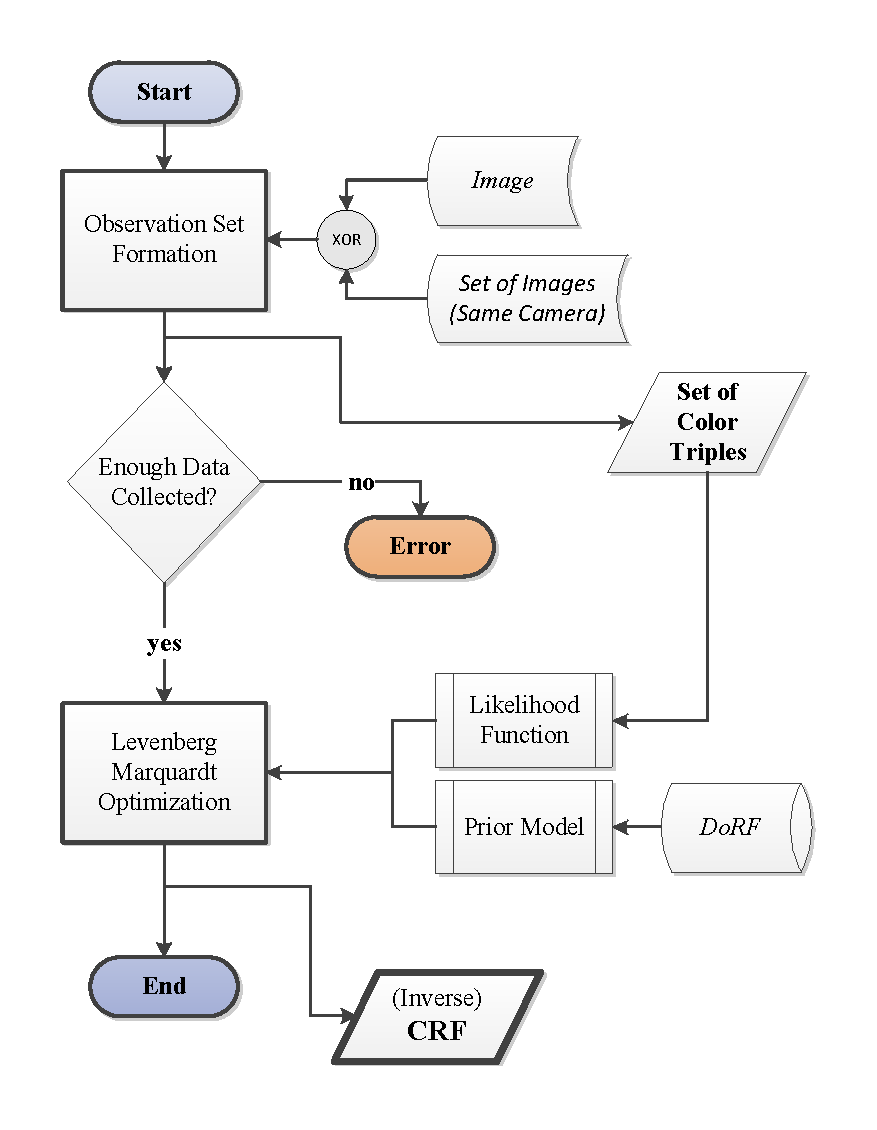
\includegraphics[width=0.9\textwidth]{images/radcal_overview.pdf}
	\caption[Flow chart (Radiometric Calibration)]{Flow chart of the algorithm. All important steps are presented in chronological order. Datasets and databases as well as the input and output of the algorithm are shown on the right.}
	\label{fig:radcaloverview}
\end{figure}

\subsubsection{Observation Set Formation}
\label{subsubsec:osf}
At first, image specific data is collected by analyzing either a single RGB image or sequentially a set of RGB images from the same camera with fixed settings. The method is based on \emph{edge} color distributions, so for locating potentially useful patches in the image, an edge image is created from the original image using the Canny operator \cite{canny1987computational}. The algorithm looks for patches of a certain fixed size $W \times H$ which are divided by an edge into exactly two regions of similar size. Like the choice of the author of this method, in this thesis the patches are squared, \hbox{i.e.} $W = H$, and unless differently stated, $W = H = 15$ pixels. As a candidate for the observation set $\Omega$, the considered patch has to meet the following conditions:
\begin{itemize}
	\item there is only one single, continuous edge path inside the patch,
	\item the color variance inside a region has to be below a specific threshold $\epsilon_\text{max}$,
	\item there has to be a minimum distance $\epsilon_\text{min}$ between the two region colors $C_1$ and $C_2$ and
	\item there are no spatially overlapping patches inside the observation set.
\end{itemize}
\begin{figure}
	\centering
	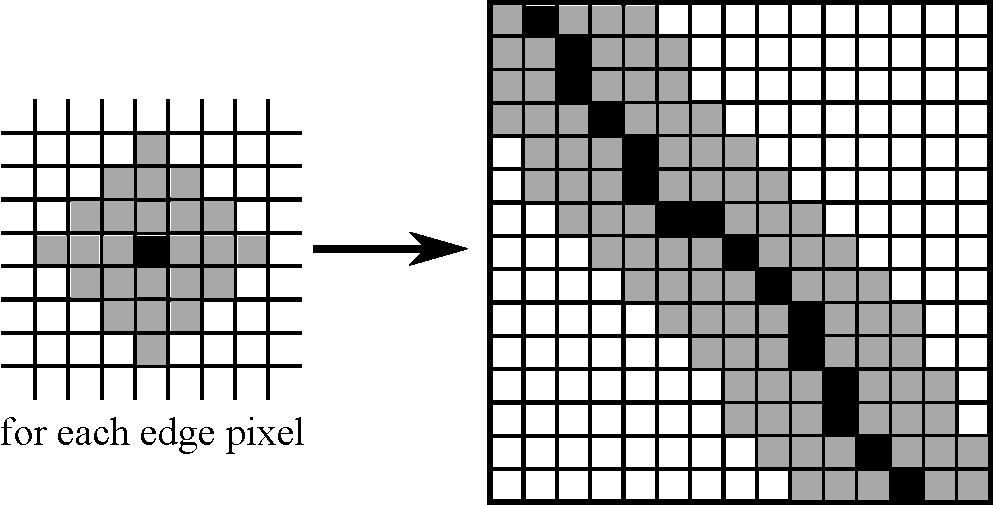
\includegraphics[width=0.5\linewidth]{images/dilation_illustration.pdf}
	\caption[Illustration of edge path dilation]{Illustration of edge path dilation. The size of the examined patch (right figure) is $15 \times 15$ pixels. Each cell in the array depicts one pixel. The edge path is given by the edge pixels (black). The dilation pixels are gray. The maximum distance from the dilation pixels to the edge path is set to 3 pixels. An example for the dilation for a single edge pixel is shown on the left.}
	\label{fig:dilationillustration}
\end{figure}
Due to the usually smooth transition from $C_1$ to $C_2$ over the edge path, the path is dilated by a few pixels, dependent on the chosen patch size $W \times H$. For patches of size $15 \times 15$ pixels, the maximum distance of each dilation pixel to the edge path has been experimentally set to 3 (for an illustration see \autoref{fig:dilationillustration}). 

Completely uniform region colors are usually very rare. Even if there is such a perfect region in scene radiance, the output of the CCD sensor is typically noisy. Hence, the finally used measurements for the region colors $C_1$ and $C_2$ are obtained by computing the mean colors inside the respective region, without considering the \emph{dilation pixels}. For each patch, several $C_{\text{edge}}$ values are available, depending on the amount of edge pixels -- or in other words -- on the length of the edge path. So more than just one \emph{edge color triple} ($C_1$, $C_2$ and $C_{\text{edge}}$) is generated for every patch by randomly choosing five of the colors on the edge path. After examining all $W \times H$ sized patches in the image or in the set of images, the data acquisition step is completed. Hence, the entire set of edge color triples $\Omega$ is compiled. A sample result of this \emph{observation set formation} is shown in \autoref{fig:patchselection} on page \pageref{fig:patchselection}. 

\begin{figure}[p]
  \centering
  \subfigure[Original image]{
    \label{subfig:patchimageorig}
    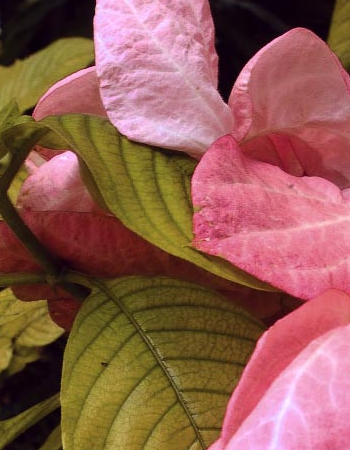
\includegraphics[width=0.45\textwidth]{images/image_for_patches_orig.png} 
  }
  \subfigure[Edge image with selected patches]{
    \label{subfig:patchimageedges}
    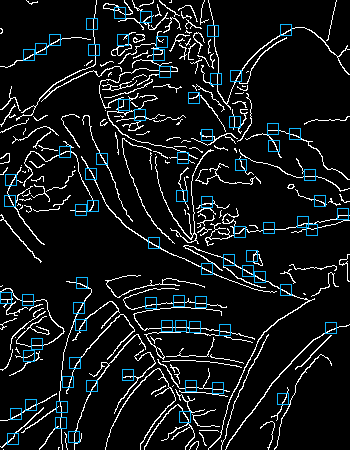
\includegraphics[width=0.45\textwidth]{images/image_for_patches_edge.png} 
  }
  \subfigure[Sample patch 1]{
    \label{subfig:samplepatch1}
    
\includegraphics[width=0.22\textwidth]{images/patches/patch44-100.png} 
  }
  \subfigure[Sample patch 2]{
    \label{subfig:samplepatch2}
    
\includegraphics[width=0.22\textwidth]{images/patches/patch195-16.png} 
  }
  \subfigure[Sample patch 3]{
    \label{subfig:samplepatch3}
    
\includegraphics[width=0.22\textwidth]{images/patches/patch70-242.png}  
  }
  \subfigure[Sample patch 4]{
    \label{subfig:samplepatch4}
    
\includegraphics[width=0.22\textwidth]{images/patches/patch294-34.png}  
  }
  \caption[Selection of appropriate edge patches]{Selection of appropriate edge patches with patch size $12 \times 12$ pixels. The top left image is the original image. On the top right side, the Canny detected edge image is shown. The blue rectangles frame all selected patches. \autoref{subfig:samplepatch1} to \autoref{subfig:samplepatch4} are the enlarged image areas of four of these detected patches.}
  \label{fig:patchselection}
\end{figure}
Now if $\left|\Omega\right|$, the amount of collected edge color triples, is zero or below a specific threshold, the subsequent optimization step will most likely not lead to robust results and thus the algorithm terminates.

\subsubsection{Bayesian Solution Method}
As seen before, the method involves both, the previously collected image specific information $\Omega$ through the point-to-line distance measurement presented in \autoref{eq:distancepointtoline} (represented by $D(g;\Omega)$) and prior knowledge on (inverse) CRFs. The latter is extracted from the DoRF database and modeled by the so-called \emph{prior model}. So the optimal inverse CRF triple $g^*$ is defined as
\begin{equation}
	g^* = \mathrm{argmax} \ p(g|\Omega) = \mathrm{argmax} \ p(\Omega|g) \cdot p(g) \enspace ,
	\label{eq:optrespfunc}
\end{equation}
where $p(\Omega|g)$ is the likelihood function from \autoref{eq:likelihoodfunction} and $p(g)$ the prior from the prior model in \autoref{eq:priormodel}. Due to the fact that $g$ is now an inverse CRF triple instead of a function for just a single channel, the prior is computed by multiplying $p(x), x \in \{g_{\text{red}}, g_{\text{green}}, g_{\text{blue}}\}$ and then taking the result to the power of $1/3$.
After a logarithmic transformation of \autoref{eq:optrespfunc} to a minimization problem, the optimization is done by an implementation of the Levenberg-Marquardt (LM) algorithm \cite{WWW:lmfit}, incorporating the objective function $E(g)$.
\begin{equation}
	g^* = \mathrm{argmin} \  E(g);\ \ \ E(g) = \lambda \cdot D(g;\Omega) - \log p(g)
	\label{eq:levmar}
\end{equation}
Note that by definition $g = g_{\text{mean}} + \vec{c} \cdot H$. $\vec{c}$ is initialized with zeros, so the optimization starts from $g_{\text{mean}}$ for all three channels (see \autoref{eq:crfconcisedescriptorPCA}). The author of the method proposes a greedy local refinement in each dimension separately after the LM algorithm converged. In our experiments, it turned out, that this step can be very time consuming without leading to significant improvements.






\clearpage

%%%%%%%%%%%%%%%%%%%%%%
% Geometry Invariants
%%%%%%%%%%%%%%%%%%%%%%

\section{Using Geometry Invariants for CRF Estimation}
\label{sec:geoinv}
Ng et \hbox{al.} proposed a novel approach for CRF estimation \cite{ng_cvpr07} in 2007, where first order geometry invariants of images are exploited. For instance, this approach is used in \cite{hsu2007image} to extract camera-specific features from segmented regions in an image. Spliced images can be detected by this method.

\subsection{Theoretical Foundation}
\label{subsec:geoinvtheory}

\subsubsection{Geometry Invariants}
\label{subsubsec:geoinv}
It is shown that by taking the partial derivative of the image intensity $R(x,y)$, properties can be extracted which are solely dependent on the CRF $f$. These are called \emph{geometry invariants}. 

$R(x,y)$ is defined as $R(x,y) = f(r(x,y))$. So taking the first order partial derivative leads to
\begin{equation}
	\Delta R(x,y) = (\ R_x \ \ R_y\ ) = f'(r) \cdot (\ r_x \ \ r_y\ ) \enspace ,
	\label{eq:1storderpartderiv}
\end{equation}
where $R_x$ and $R_y$ denote the first order partial derivatives of image intensity in $x$- and $y$-direction. Note that they are products of two factors each. For both, the first factor is $f'(r)$, which is only related to the CRF. The second factors, $r_x$ and $r_y$, are the first order partial derivatives in $x$- and $y$-direction in the domain of image irradiance. They are purely related to the image geometry. In the following steps it is shown, that the effects of image geometry in $r_x$ and $r_y$ can be removed by mathematical transforms and constraints. For reasons of clarity and comprehensibility, the derivation is only for $R_x$ shown, $R_y$ is analogously derived.

Let $R_x$ and $R_{xx}$ the first and second order partial derivative in $x$-direction.
\begin{equation}
	R_x = f'(r) \cdot r_x
	\label{eq:Rx}
\end{equation}
\begin{equation}
	R_{xx} = f''(r) \cdot r_x^2 + f'(r) \cdot r_{xx}
	\label{eq:Rxx}
\end{equation}
Due to the fact that $r(x,y)$ is an arbitrary function and thus the elimination of its geometric component is a difficult task, Taylor expansion is used to approximate the local geometry. The class of planar surfaces is mathematically defined as
\begin{equation}
	\left\{\ r(x,y) : r(x,y) = a \cdot x + b \cdot y + c;\ \ a,b,c \in \mathbb{R}\ \ \right\} \enspace .
	\label{eq:classofplanarsurfaces}
\end{equation}
The equation $r_{xx} = r_{xy} = r_{yy} = 0$ holds for those planes, where $r_{xy}$ is the partial derivative in $x$- and $y$-direction. Consequently, for planes the second order partial derivative $R_{xx}$ from \autoref{eq:Rxx} can be simplified to
\begin{equation}
	R_{xx} = f''(r) \cdot r_x^2 + \underbrace{f'(r) \cdot r_{xx}}_{= \ 0} = f''(r) \cdot r_x^2 \enspace .
	\label{eq:Rxxsimplified}
\end{equation}
Then, by incorporating \autoref{eq:Rx} and \autoref{eq:Rxxsimplified}, the geometry component $r_x$ can be removed, such that
\begin{equation}
	\frac{R_{xx}}{R_x^2} = \frac{f''(r) \cdot r_x^2}{(f'(r) \cdot r_x)^2} = \frac{f''(r) \cdot r_x^2}{(f'(r))^2 \cdot r_x^2} = \frac{f''(r)}{(f'(r))^2} \enspace .
	\label{eq:Rxxalmostdone}
\end{equation}
Using the definition of image irradiance $r = g(R) = f^{-1}(R)$, \autoref{eq:Rxxalmostdone} can be rewritten as
\begin{equation}
	\frac{R_{xx}}{R_x^2} = \frac{f''(f^{-1}(R))}{(f'(f^{-1}(R)))^2} \ \dot{=} \ G_1(R) \enspace ,
	\label{eq:Rxxdone}
\end{equation}
where for a particular CRF and a fixed image intensity value $R(x,y)$, $G_1(R)$ -- characterized as ``quantities that are invariant to the class of planar surfaces'' -- is a constant, independent from the first order geometry of image irradiance $r$.

Hence, at this step the effect of image geometry is completely eliminated. Note that \autoref{eq:Rxxdone} consists only of terms related to the CRF $f$ and to the image intensity $R$. As mentioned before, the same mathematical derivation can be applied to the first order partial derivative in $y$-direction $R_y$, but also $R_{xy}$ can be transformed to the first order geometry invariant $G_1$. All these results combined are presented in the following.
\begin{equation}
	\underbrace{\frac{R_{xx}}{R_x^2} = \frac{R_{yy}}{R_y^2} = \frac{R_{xy}}{R_x R_y}}_{\text{derivative equality constraint}} = \frac{f''(f^{-1}(R))}{(f'(f^{-1}(R)))^2} \ \dot{=} \ G_1(R) \enspace ,
	\label{eq:RxxandRyyandRxy}
\end{equation}
where -- due to their implication of important geometric properties -- the first two equality constraints are pointed out above and are referred to as \emph{derivative equality constraints} as from now. One of these properties of $G_1$ is its invariance to affine transformations, so that the value of $G_1$ is preserved under local coordinate frame rotation. This helps to overcome some implementation difficulties (see \autoref{subsec:geoinvalgo}). 

In theory, the inverse CRF $g$ can be computed by solving an integral
\begin{equation}
	g(R) = f^{-1}(R) = \int{\exp \left(-\int{G_1(R)\delta R} \right) \delta R} \enspace ,
	\label{eq:integralsolution}
\end{equation}
which can be derived from the last equality relation of \autoref{eq:RxxandRyyandRxy}. But in practice, the feasibility of this analytical approach is limited by the measuring accuracy of the camera sensor. This affects the precision of the computation of the derivatives.

For the analytical estimation, the camera response curve is approximated by a model. One of the earliest CRF models is the gamma curve model
\begin{equation}
	f(r) = r^{\gamma} \text{ and } \ g(R) = R^{\frac{1}{\gamma}} \enspace ,
	\label{eq:gammacurves}
\end{equation}
where $\gamma$ is the model-specific parameter.

Considering this model, it is shown, that $G_1$ has a simple relationship with $\gamma$, expressed through $Q(R)$.
\begin{equation}
	G_1(R) = \frac{\gamma - 1}{\gamma \cdot R}; \ \ \gamma = \frac{1}{1-G_1(R) \cdot R}\ \dot{=}\ Q(R)
	\label{eq:G1RtoQR}
\end{equation}
Note that the expression $Q(R)$ can also be computed and used when having more complex curves than pure gamma curves as is the case with most real-word CRFs.

\subsubsection{Generalized Gamma Curve Model}
\label{subsubsec:ggcm}
The latter and the fact, that gamma curves have only a very limited fitting capability to real-world CRFs, motivates the proposition of a more complex model, the generalized gamma curve model (GGCM):
\begin{equation}
	f(r) = r^{P(r, \vec{\alpha})} \text{ and } g(R) = R^{\frac{1}{P(R, \vec{\alpha})}} \enspace ,
  \label{eq:ggcm}
\end{equation}
where $\vec{\alpha} = \left[\alpha_0,...,\alpha_n\right]$ is a $(n+1)$-dimensional coefficient vector for the $n$-th order polynomial $P(x,\vec{\alpha}) = \sum_{i=0}^n\alpha_i \cdot x^i$. This model is just an extension to the original gamma curve model, because it can be reduced to the latter by setting $n = 0$, so that $P$ only consists of a constant term $\alpha_0 = \gamma$. Then, 
\begin{equation}
	P(x, \vec{\alpha}) = \sum\limits_{i=0}^0\alpha_i \cdot x^i = \alpha_0 \cdot x^0 = \alpha_0\ \dot{=}\ \gamma \enspace .
	\label{eq:reducePtoconstant}
\end{equation}
Ng et \hbox{al.} compared the analytical GGCM to the empirical EMoR model from \cite{CAVE_0091} and to the analytical polynomial model proposed in \cite{CAVE_0068}. They applied least square fit to the 201 CRFs in DoRF. It turned out that GGCM only performs slightly worse then the EMoR model, but has a much smaller error in comparison to the polynomial model. That makes GGCM a good choice for this analytical approach on CRF estimation.


\clearpage

\subsection{The Algorithm}
\label{subsec:geoinvalgo}
Given an image $I$, the first order partial derivatives of image intensity $\widetilde{R}_x$ and $\widetilde{R}_y$ are computed. Then for each pixel in $I$, its local neighborhood is temporarily rotated by $(\mathrm{arctan}(\frac{\widetilde{R}_y}{\widetilde{R}_x}) \cdot \frac{180^\circ}{\pi} + 45^\circ)$ to compute the first to second order partial derivatives $R_x$, $R_y$, $R_{xx}$, $R_{yy}$ and $R_{xy}$. The rotation is done to overcome singularity problems. Then, for every pixel in $I$, an error function
\begin{equation}
	E(R) = \left|\frac{R_{xx}}{R_x^2} - \frac{R_{yy}}{R_y^2}\right| + 
				 \left|\frac{R_{xx}}{R_x^2} - \frac{R_{xy}}{R_x \cdot R_y}\right| + 
				 \left|\frac{R_{yy}}{R_y^2} - \frac{R_{xy}}{R_x \cdot R_y}\right|
	\label{eq:errorfunction}
\end{equation}
is evaluated, which is strongly related to the derivative equality constraint (\autoref{eq:RxxandRyyandRxy}). If the value of $E(R)$ is below a specific threshold $\epsilon$, e.g. $\epsilon = 10$ as proposed in the paper, the pixel is considered a candidate point for the set of \emph{locally planar irradiance points} $S_\text{LPIP}$ and thus taken into the set of locally linear isophote points $S_\text{LISO}$, of which $S_\text{LPIP}$ is a subset. For differentiating the real LPIPs from those, which are not locally planar in the irradiance domain, Bayesian inference is utilized.

\subsubsection{Bayesian Inference}
\label{subsubsec:naivebayes}
For extracting the common characteristics of LPIPs, two kinds of features are used, derivative geometric quantities and three moment features ($m_0$, $m_1$ and $m_2$) based on a small neighborhood in the binary LISO map $b(x,y)$, where $b(x,y) = 1$ if and only if the pixel corresponding to the coordinates $(x,y)$ is in $S_\text{LISO}$, otherwise $b(x,y) = 0$. For an example of a LISO map see \autoref{fig:lisomap} on page \pageref{fig:lisomap}. 
\begin{figure}[htbp]
  \centering
  \subfigure[Original image]{
    \label{subfig:imgallchannels}
    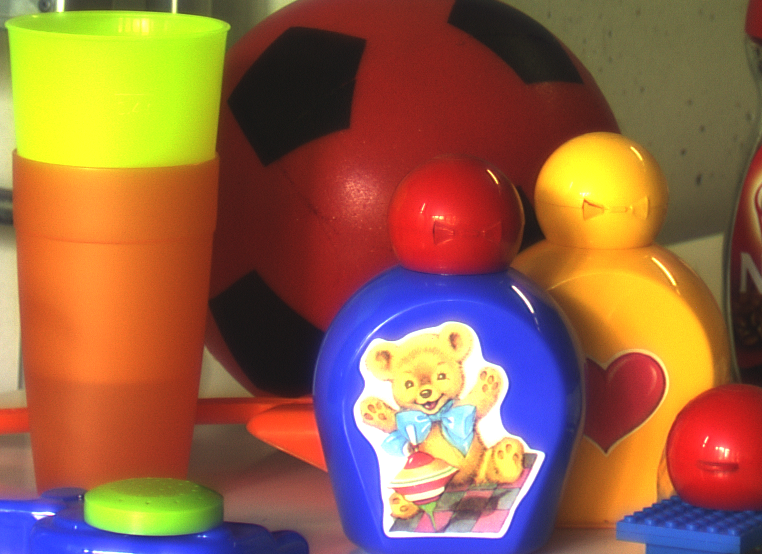
\includegraphics[width=0.45\textwidth]{images/img_all_channels.png} 
  }
  \subfigure[Extracted red channel]{
    \label{subfig:imgredchannel}
    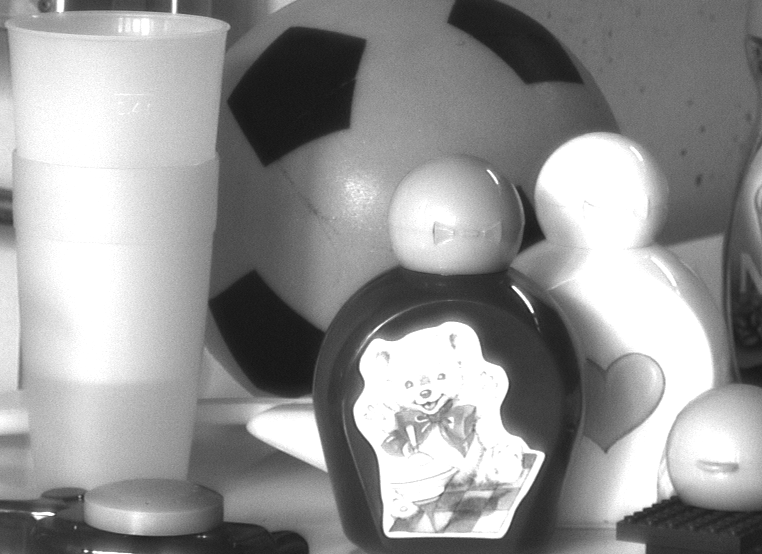
\includegraphics[width=0.45\textwidth]{images/img_red.png} 
  }
  \subfigure[Computed LISO map]{
    \label{subfig:lisomapred}
    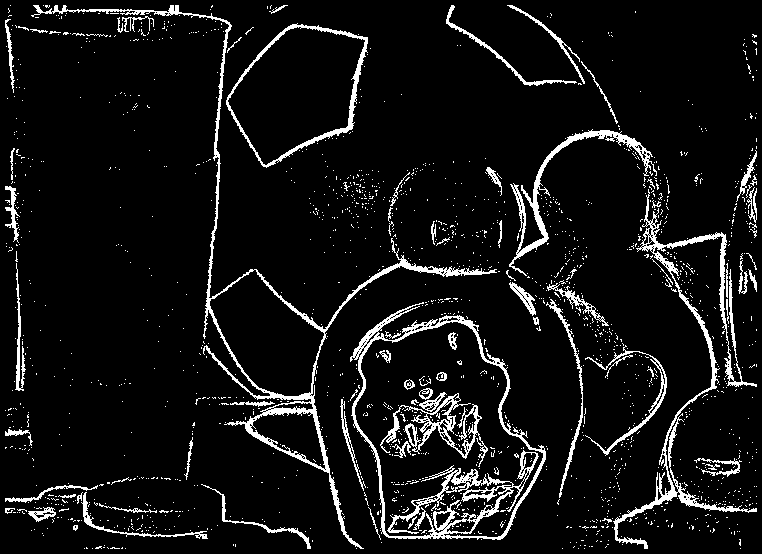
\includegraphics[width=0.8\textwidth]{images/liso_map_red.png} 
  }
  \caption[Example for a LISO map]{Example for a LISO map. \autoref{subfig:imgallchannels} shows the original image. In \autoref{subfig:imgredchannel} only the red channel is shown, which is used by the algorithm to generate the binary LISO map for the particular channel. The LISO map is shown in \autoref{subfig:lisomapred}. Note that most of the points in the LISO set lie around edges in the image.}
  \label{fig:lisomap}
\end{figure}
All in all, six features have to be computed:
\begin{itemize}
	\item error function value $E(R)$,
	\item gradient magnitude $\left|\mathrm{grad}(R)\right| = \sqrt{R_x^2+R_y^2}$\ ,
	\item normalized second derivative in gradient direction $\lambda = \frac{R_{gg}}{R_g^2}$, where $R_g$ and $R_{gg}$ are the first and second order partial derivatives in gradient direction,
	\item total mass $m_0 = \sum\limits_{(x,y)\in N_5} b(x,y)$, where $N_5$ denotes a $(5 \times 5)$ pixels neighborhood window,
	\item centroid $m_1$ and
	\item radius of gyration $m_2$.
\end{itemize}

For the training of the Bayes classifier, a set of training images is compiled by using either linear real-world or linear synthetic images and then applying different gamma curves with $\gamma \in [0.2; 0.6]$. 

As seen before, gamma curves are horizontal lines in $Q$-$R$ space, and so all points in $S_\text{LISO}$ are classified into $S_\text{LPIP}$ and $S_\text{non-LPIP}$ by the following criterion.
\begin{equation}
	(x,y) \in 
	\begin{cases}
	  S_\text{LPIP}				&\text{if} \ \ \left|Q(x,y) - \gamma\right| \leq 0.1 \\
	  S_\text{non-LPIP}		&\text{else}
	\end{cases}
	\label{eq:lpipclassification}
\end{equation}
Hence, all points in $S_\text{LPIP}$ have a $Q$ value close to $\gamma$. 

Let $c \in \left\{S_\text{LPIP}, S_\text{non-LPIP}\right\}$. Then $P(c) = \frac{\left|c\right|}{\left|S_\text{LISO}\right|}$, where $\left|\cdot\right|$ denotes the number of elements in a class. Therefore, $P(c)$ is the ratio of points belonging the the class $c$. The a-posterior probability of a LISO being a LPIP is then given by
\begin{equation}
	P(S_{LPIP}| \vec{f}) = 
	\frac{P(\vec{f}|S_\text{LPIP}) \cdot P(S_\text{LPIP})}{P(\vec{f}|S_\text{LPIP}) \cdot P(S_\text{LPIP}) + P(\vec{f}|S_\text{non-LPIP}) \cdot P(S_\text{non-LPIP})} \enspace ,
	\label{eq:aposterior}
\end{equation}
where $\vec{f} = [f_1, ..., f_6]$ is the six-dimensional feature vector containing the computed feature values. Let $h(c, i, v)$ the ratio of elements belonging to the respective bin for the feature value $v$ in the histogram of the $i$'th feature of the class $c$ over the entire number of elements in $c$. $P(\vec{f}|c)$ is then given by
\begin{equation}
	P(\vec{f}|c) = \prod\limits_{i=1}^{6} \frac{h(S_\text{LPIP}, i, f_i)}{h(S_\text{LPIP}, i, f_i) + h(S_\text{non-LPIP}, i, f_i)} \enspace .
	\label{eq:featureratios}
\end{equation}

The conditional probability function $P(S_\text{LPIP}| \vec{f})$ from \autoref{eq:aposterior} is used as a weighting function for the points in $S_\text{LISO}$, when it comes to the actual CRF estimation. The weighted \hbox{$Q$-$R$} histogram is also referred to as \emph{CRF signature} in Ng's subsequent publications \cite{ng_wifs09_1} and \cite{ng_wifs09_2}.


\clearpage

\subsubsection{CRF Estimation}
\label{subsubsec:CRFestimation}
As presented in \autoref{subsec:geoinvtheory}, the CRF estimation method is based on the GGCM model. Due to the tradeoff between modeling power and computational complexity, a first order GGCM \hbox{($n = 1$)} is used. Hence, the coefficient vector $\vec{\alpha} = \left[\alpha_0, \alpha_1\right]$ is only two-dimensional. Nevertheless, the model exhibits good fit to real-world CRFs in comparison to a purely polynomial model. 

Let $N = |S_\text{LISO}|$ and $Q_n$, $R_n$ and $\vec{f}_n$ the $Q$- and $R$-value and feature vector of the $n$-th element in $S_\text{LISO}$. The best possible coefficient vector $\vec{\alpha}^*$ can be determined by minimizing the objective function
\begin{equation}
	\vec{\alpha}^* = \mathrm{argmin} \ \sum\limits_{i = 1}^{N}{ \frac{P(S_{LPIP}| \vec{f}_i)}{P(R_i)} \ \left|Q_i - \widetilde{Q}(R_i,\vec{\alpha})\right|^2 } \enspace .
	\label{eq:objectivefunction}
\end{equation}
$P(R)$ is the ratio of points with this particular intensity value over all points in $S_\text{LISO}$. It is utilized to overcome polarization effects during the optimization, if the distribution of $R$ is unbalanced in the image. Given an inverse CRF $g_{\vec{\alpha}}$, where $\vec{\alpha}$ is the coefficient vector for GGCM, $\widetilde{Q}$ determines the $Q$-value corresponding to $R$,
\begin{equation}
	\widetilde{Q}(R, \vec{\alpha}) = \frac{g_{\vec{\alpha}}'(R)}{1 + g_{\vec{\alpha}}''(R) \cdot R} \enspace .
	\label{eq:Qtilde}
\end{equation}

\vspace{1cm}

\subsubsection{Refinement}
\label{subsubsec:refinement}

Ng et \hbox{al.} propose an additional refinement by a calibration, when linearizing $Q(R)$ with respect to the differential change of the gamma curve parameter $\gamma$:
\begin{equation}
	\overline{Q}(R) = \frac{\sqrt{3}}{\sqrt{3} - 1} \left(1 - \sqrt{1 - \frac{1}{2 \cdot Q(R)+1}}\ \right) \enspace .
	\label{eq:calibration}
\end{equation}
Note that every $Q$-value has to be computed this way for the refinement to take effect.    % (\chapter{})
\cleardoublepage
\chapter{Evaluation}
\label{chap:evaluation}


\section{Challenges}
\label{sec:challenges}

\subsection{CRF-dependent Distribution of Q-Values}
\label{subsec:crfdependentdistributionofQvalues}

The implementation of \cite{ng_cvpr07} has issues, which we were not able to solve. The problems show up first, when examining our created $Q$-$R$ histograms. The failure could be detected by computing these histograms for several images with known ground-truth CRFs. The distribution of the $Q$-values did not shift as predicted in theory. How these observations were obtained is described in the following.

Both, real-world and synthetic images were examined, and similar results were obtained. The real-world data was obtained by extracting linear RAW images from a camera and then manually applying a gamma function with different parameters $\gamma \in \left\{ 0.2, 0.4, 0.6, 0.8 \right\}$. For synthetic images, many -- about 1500 -- randomly sized filled circles with a random intensity each are put into an empty image. This image is then scaled up using bilinear interpolation to make the edges less sharp. As with real-world images, gamma curves were applied afterwards to mimic the camera response of a usual digital camera.

In theory, for $Q(R)$ histograms of images with mainly uniform distributed irradiance values,
\begin{enumerate}
	\item the mean intensity value $R_\text{mean}$ over all points in $S_\text{LISO}$ increases with decreasing $\gamma$. The reason is, that for instance for $\gamma = 0.2$, for small $R$ (low intensity values), the gamma curve $R = f(r) = r^{0.2}$ has a much larger slope than curves with larger $\gamma$. Remember, that $r \in [0; 1]$. Consequently, $R_\text{mean}$ increases. The second expected observation is, that
	\item $Q_\text{mean}$, similarly defined as $R_\text{mean}$, is smaller for small $\gamma$ than for large $\gamma$, because $Q(R)$ is directly related to the gamma curve parameter $\gamma$ (see \autoref{subsec:geoinvtheory}).
\end{enumerate}

The effects of the first assumption could be observed in all of our tests. Let $\gamma_1 < \gamma_2$. Then the distribution of $Q(R)$-values for histograms computed over images with $\gamma_1$ significantly shifts horizontally to the right (larger intensity values) in contrast to histograms computed over images with $\gamma_2$. Four example histograms for real-world images are presented in \autoref{fig:gamma_hists}.

\begin{figure}[tb]
	\centering
		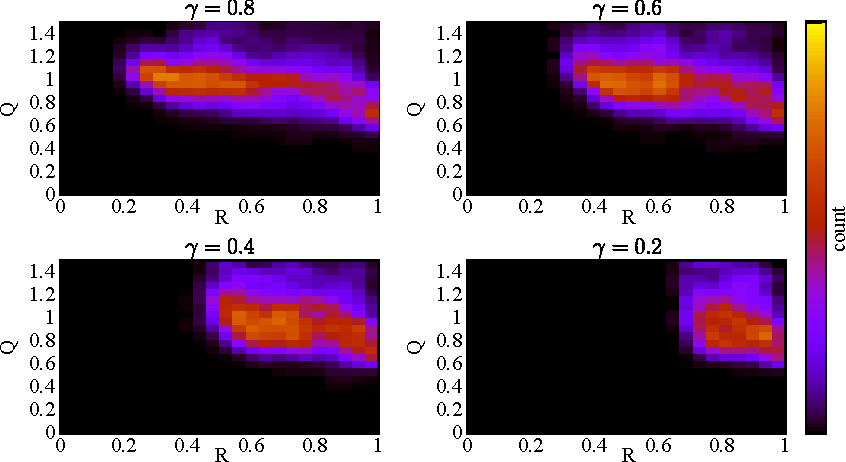
\includegraphics[width=0.95\textwidth]{histograms/geoinv_QR-diagramme.pdf}
	\caption[$Q$-$R$ histograms computed over images for different $\gamma$ curves]{$Q$-$R$ histograms computed over linear images, on which different gamma curves were applied. The upper left histogram shows the distribution of $Q(R)$-values for the largest value of $\gamma$. In the lower right, the $\gamma$-value is very small. Dark colors mean a low amount of occurring $Q(R)$-values in this area, while bright (yellow) colors stand for clusters corresponding to many $Q(R)$-values in $S_\text{LISO}$.}
	\label{fig:gamma_hists}
\end{figure}

But the second assumption turned out to be false for our implementation. The distribution of the $Q$-values does not shift vertically in the presented histograms, \hbox{i.e.} the $Q$-$R$ distribution does not align to the ground truth $\gamma$-line. The vertical distribution is very similar for all presented histograms, although $\gamma$ significantly differs.

Similar observations for both assumptions were obtained for all tested images. Hence, for instance for small values of $\gamma$, having almost no $Q$-values nearby the ground-truth, the subsequent optimization step fails consequently. The reason is, that it is heavily dependent on a reliable amount of properly detected points in $S_\text{LISO}$.



\clearpage

\subsection{Examination of Bayesian Inference}
\label{subsec:examinationofbayesianinf}

Another crucial part is the weighting of the points in $S_\text{LISO}$ as presented in \autoref{subsubsec:naivebayes}. Despite the problems with the $Q$-$R$-distribution described in \autoref{subsec:crfdependentdistributionofQvalues}, some of our obtained feature histograms appear quite similar to those presented in Ng's publication, but also significant mismatches were observed.

To create the feature histograms, we used a similar approach to the one in the previous section, gamma curves with $\gamma \in \left\{0.2, 0.4, 0.6\right\}$ were applied to both, synthetic and real-world images. Then the algorithm as presented in \autoref{subsec:geoinvalgo} is applied. Now we have $Q(R)$-histograms similar to those in \autoref{fig:gamma_hists}. These histograms represent the distribution of $Q(R)$-values over all points in $S_\text{LISO}$. Hence, this set of points is then classified into $S_\text{LPIP}$ and $S_\text{non-LPIP}$ by utilizing \autoref{eq:lpipclassification}. This procedure is repeated several times for different images and $\gamma$-values, resulting in two large sets of LPIPs and non-LPIPs, by concatenating all obtained $S_\text{LPIP}$ and $S_\text{non-LPIP}$. 

Due to the fact that the number of elements in $S_\text{LPIP}$ can significantly differ to $\left|S_\text{non-LPIP}\right|$, both sets are normalized to $[0; 1]$. This makes the histograms of $S_\text{LPIP}$ more comparable to the histograms of $S_\text{non-LPIP}$. The specific range of each feature is divided into a reliable number of bins and the normalized number of observations (points) per bin is stored. 

Our results are presented on page \pageref{fig:featurehistograms}. \autoref{fig:featurehistograms} shows the normalized histograms computed over more than 15 RAW images extracted from Hitachi HV-F22F. \autoref{fig:featurehistogramssynthetic} shows the normalized histograms of synthetic images.

The main differences to Ng's histograms are:
\begin{itemize}
	\item for small error values $E(R)$, our amplitude of non-LPIPs is significantly larger than Ng's. There, the histograms for the the two classes are even quite similar in contrast to those in \autoref{subfig:er} or \autoref{subfig:ersynthetic}.
	\item Also the second feature does not differ a lot for LPIPs and non-LPIPs in the paper, while our histograms are relatively dissimilar.
	\item The values of the third feature in \autoref{subfig:lambda} and \autoref{subfig:lambdasynthetic} range from negative to positive values, whereas in the paper, the values for this feature are all negative ($< 0$).
\end{itemize}

\begin{figure}[tbp]
  \centering
  \subfigure[Error function value $E(R)$]{
    \label{subfig:er}
    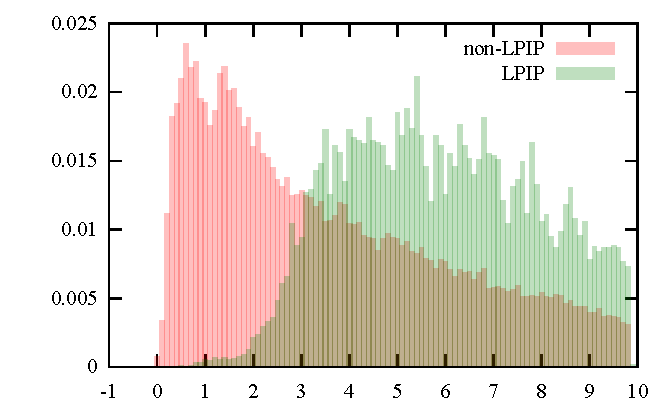
\includegraphics[width=0.31\textwidth]{plots/feature0.pdf} 
  }
  \subfigure[Gradient magnitude $\left|\mathrm{grad}(R)\right|$]{
    \label{subfig:gradientmagnitude}
    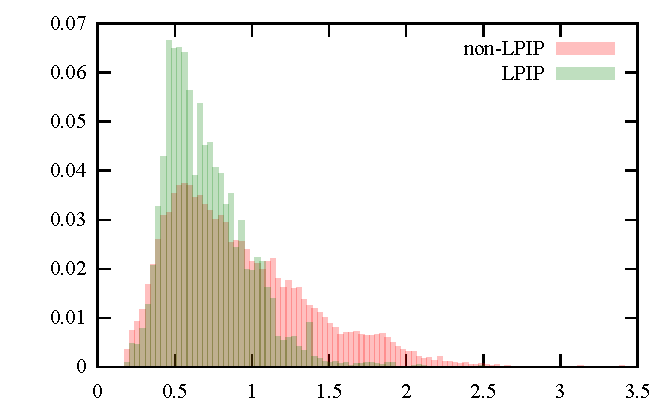
\includegraphics[width=0.31\textwidth]{plots/feature1.pdf} 
  }
  \subfigure[Lambda $\lambda$]{
    \label{subfig:lambda}
    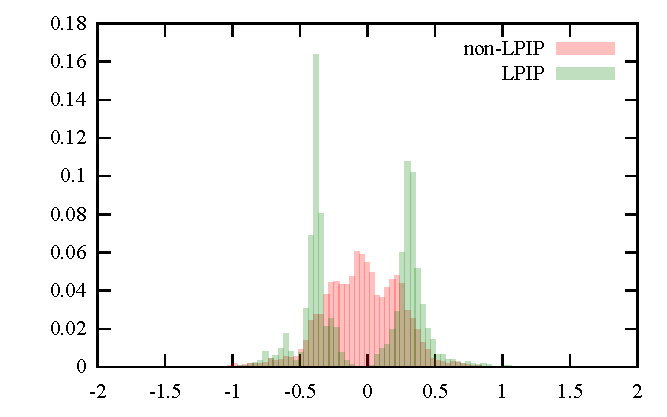
\includegraphics[width=0.31\textwidth]{plots/feature2.pdf} 
  }
  \subfigure[Total mass $m_0$]{
    \label{subfig:totalmass}
    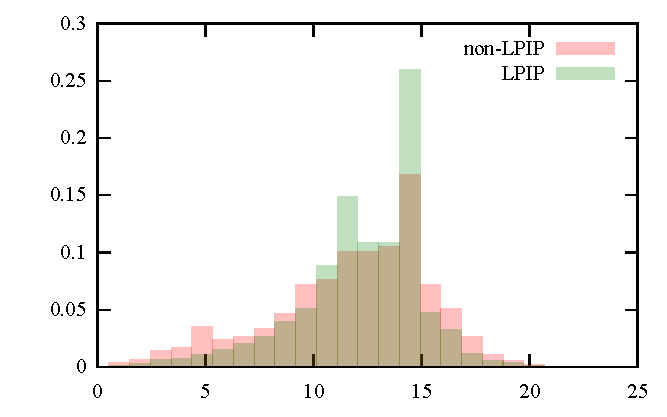
\includegraphics[width=0.31\textwidth]{plots/feature3.pdf} 
  }
  \subfigure[Centroid $m_1$]{
    \label{subfig:centroid}
    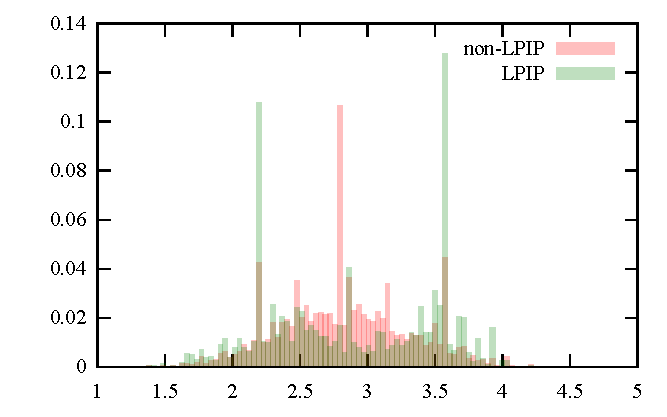
\includegraphics[width=0.31\textwidth]{plots/feature4.pdf} 
  }
  \subfigure[Radius of Gyration $m_2$]{
    \label{subfig:gyration}
    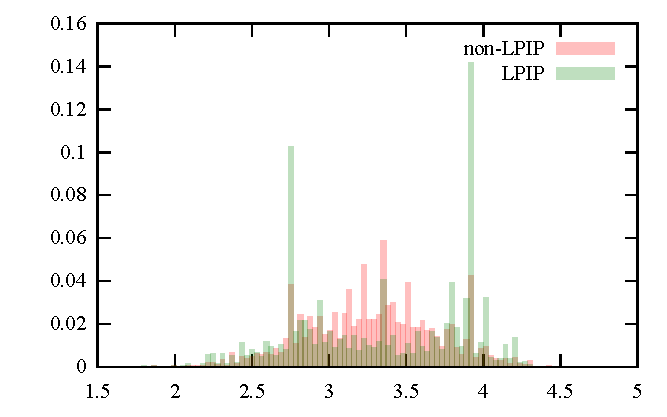
\includegraphics[width=0.31\textwidth]{plots/feature5.pdf} 
  }
  \caption{Normalized feature histograms generated with \emph{RAW} images}
  \label{fig:featurehistograms}
\end{figure}

\begin{figure}[tbp]
  \centering
  \subfigure[Error function value $E(R)$]{
    \label{subfig:ersynthetic}
    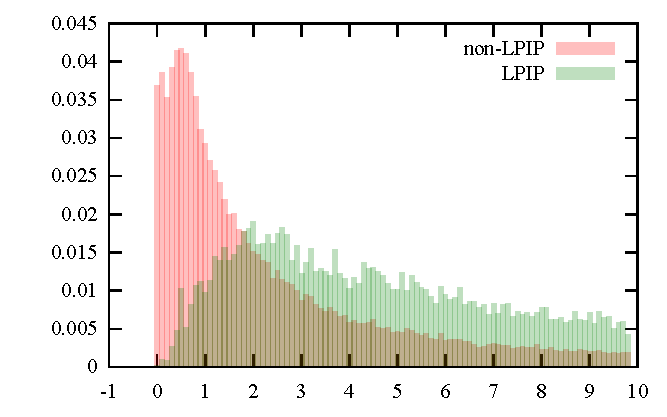
\includegraphics[width=0.3\textwidth]{plots/featureSynth0.pdf} 
  }
  \subfigure[Gradient magnitude $\left|\mathrm{grad}(R)\right|$]{
    \label{subfig:gradientmagnitudesynthetic}
    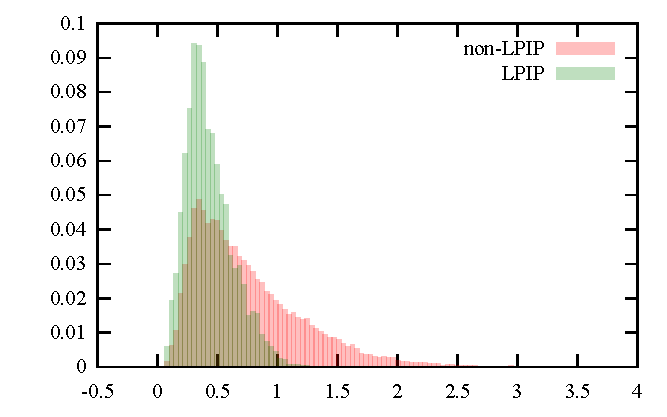
\includegraphics[width=0.3\textwidth]{plots/featureSynth1.pdf} 
  }
  \subfigure[Lambda $\lambda$]{
    \label{subfig:lambdasynthetic}
    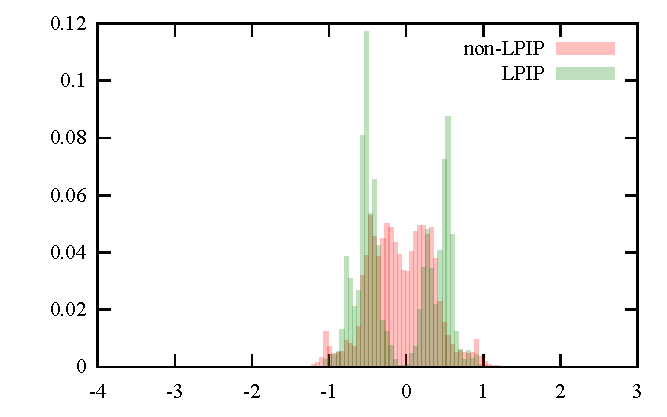
\includegraphics[width=0.3\textwidth]{plots/featureSynth2.pdf} 
  }
  \subfigure[Total mass $m_0$]{
    \label{subfig:totalmasssynthetic}
    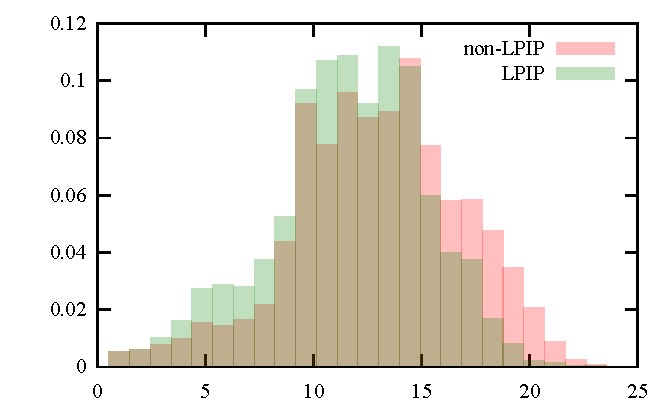
\includegraphics[width=0.3\textwidth]{plots/featureSynth3.pdf} 
  }
  \subfigure[Centroid $m_1$]{
    \label{subfig:centroidsynthetic}
    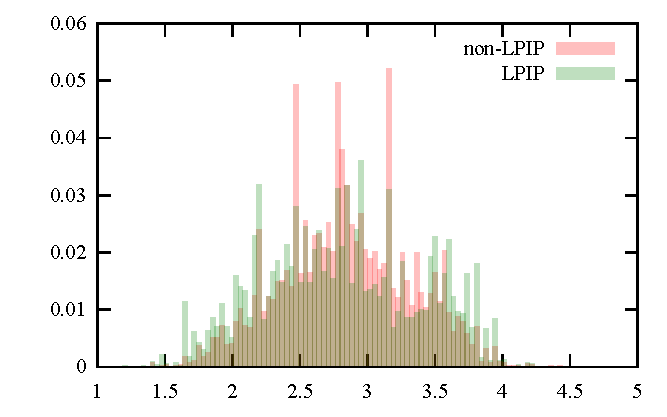
\includegraphics[width=0.3\textwidth]{plots/featureSynth4.pdf} 
  }
  \subfigure[Radius of Gyration $m_2$]{
    \label{subfig:gyrationsynthetic}
    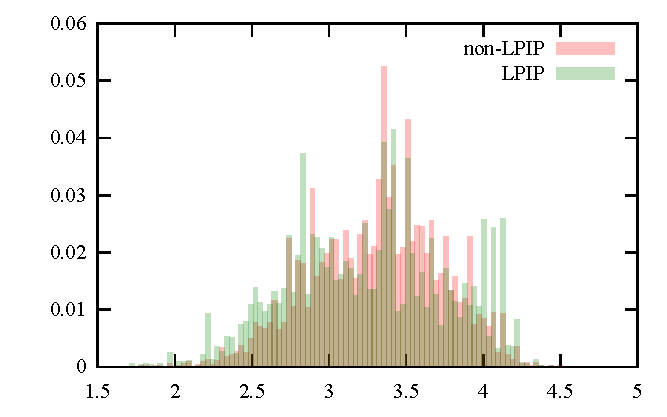
\includegraphics[width=0.3\textwidth]{plots/featureSynth5.pdf} 
  }
  \caption{Normalized feature histograms generated with \emph{synthetic} images}
  \label{fig:featurehistogramssynthetic}
\end{figure}




\clearpage

\subsection{Problem-solving Approach}
\label{subsec:problemsolving}

The main problem is described in \autoref{subsec:examinationofbayesianinf}, our implementation fails finding a reliable amount of points around the ground-truth line in $Q$-$R$ space. Consequently, the feature histograms used for the classification can not be correct. An approach for further efforts in localizing the actual error source, either a missing implementation detail or something being wrong with the theory part, is presented in the following.

For this approach, the value of the error function is ignored, \hbox{i.e.} every point is taken into $S_\text{LISO}$. Hence, all points of the image are classified into $S_\text{LPIP}$ and $S_\text{non-LPIP}$ (analogous to \autoref{eq:lpipclassification}). This is applied three times to a particular image, using three different gamma curves, where $\gamma \in \left\{0.2, 0.4, 0.6\right\}$. 

Next, the three distinct ``LPIP-maps'' (containing only the classified LPIPs at their specific position from the original image) $L_{0.2}$, $L_{0.4}$ and $L_{0.6}$ are extracted and combined afterwards. $L_{\gamma}$ denotes the LPIP-map for the particular $\gamma$. The combination is done by first creating an empty RGB image and second using the three LPIP-maps as the three channels, where $L_{0.2}$ is used as the red, $L_{0.4}$ as the green and $L_{0.6}$ as the blue channel. 

With this image, points, which are classified as LPIPs for all three gamma curves, can be extracted easily, because they appear white. In the example from \autoref{fig:LPIPmaps}, about $14 \%$ of all colored pixels fulfill this condition. Now, these points can be analyzed to get further insight.

\vspace{0.7cm}

\begin{figure}[htbp]
  \centering
  \subfigure[original image]{
    \label{subfig:original image}
    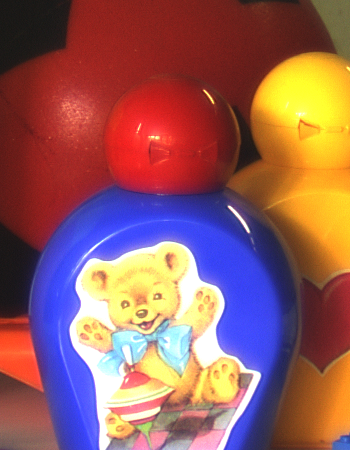
\includegraphics[width=0.315\textwidth]{liso_maps/small.png} 
  }
  \subfigure[combined LPIP-map]{
    \label{subfig:combined LPIP-map}
    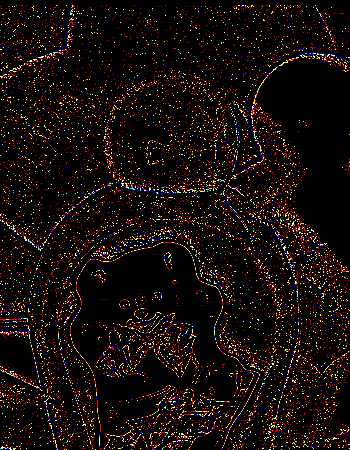
\includegraphics[width=0.315\textwidth]{liso_maps/all.png} 
  }
  \subfigure[intersection of LPIP-maps]{
    \label{subfig:white points}
    
\includegraphics[width=0.315\textwidth]{liso_maps/white_only.png} 
  }
  \caption[Original image and combined LPIP-map]{Original image, combined LPIP-map and intersection of all channels (white pixels).}
  \label{fig:LPIPmaps}
\end{figure}



\clearpage

\section{Capabilities of Data Acquisition}
\label{sec:capabilitiesofdataacqu}

In this and the next two evaluation appraoches, only the method by Lin et al. is examined. It requires a sufficienctly large, representative set of edge samples. If not enough data could be gathered before, the optimization step can not produce any good results. Hence, the data acquisition step, taking place before the actual CRF estimation algorithm, is analyzed.


\subsection{Crucial Parameters}
\label{subsec:parameterIntroduction}

Tests have shown that the amount of accepted patches and thus the size of the observation set is heavily dependent on the settings of two parameters:
\begin{enumerate}
	\item $\epsilon_\text{min}$, threshold for the minimum distance between the two region colors $C_1$ and $C_2$ and
	\item $\epsilon_\text{max}$, threshold for the maximum distance of the colors within a region $C_1$ or $C_2$.
\end{enumerate}
For all distance computations the common Euclidean norm is used, although other distance metrics are possible.

At first, the boundaries $B$ for both parameters have to be found, what is straightforward due to the use of normalized RGB colors and the Euclidean norm. All points in the three-dimensional normalized RGB space lie in a cube spanned by the unit vectors $(1, 0, 0)^\mathrm{T}$, $(0, 1, 0)^\mathrm{T}$ and $(0, 0, 1)^\mathrm{T}$ with its origin at $(0, 0, 0)^\mathrm{T}$, where $\vec{x}^\mathrm{T}$ denotes the transposed vector $\vec{x}$. Hence, the largest distance inside that cube -- considering the Euclidean norm -- is $\sqrt{1^2+1^2+1^2} = \sqrt{3} \ \ \Rightarrow \  \epsilon_\text{min}, \epsilon_\text{max} \in B = [0; \sqrt{3}]$.

Knowledge about the impact of these parameters on the dataset quality is of high relevance for a reasonable evaluation. If $\epsilon_\text{min}$, the minimum distance between $C_1$ and $C_2$ -- \hbox{i.e.} a measurement for how dissimilar the colors have to be -- is too small, the line between the region colors can also be very short. That might not be a problem in theory, but in practice, due to the computation of the region colors (just taking the mean color of all colors within a region bounded by the size of the patch and the edge inside the patch), the variance of the colors inside the region highly affects the reliability of the following CRF estimation for a small $\epsilon_\text{min}$. This variance is covered by $\epsilon_\text{max}$, thresholding the maximum Euclidean distance of the colors within a region. This can be seen as the degree of similarity of the respective colors. Hence, the obvious choice for the two parameters considering optimal conditions (no noise and regions with uniform colors) would be $\epsilon_\text{min} \rightarrow \text{max}(B) = \sqrt{3};\ \ \epsilon_\text{max} = \text{min}(B) = 0$.

The expectation on the parameters is, that they have an opposing behavior. $\epsilon_\text{max}$ is related to the number of found patches, \hbox{i.e.} the larger the value of $\epsilon_\text{max}$ gets, the more patches will be found. Large values of $\epsilon_\text{min}$ on the other hand will result in a small number of patches. 

That all leads to the conclusion, that first $\epsilon_\text{min} > \epsilon_\text{max}$ and second the difference $\epsilon_\text{min} - \epsilon_\text{max}$ should be as large as possible. Third, a sufficiently large number of patches must be extracted.  


\subsection{Color Coverage Factor}
\label{subsec:colorCoverageFactor}

Not only the number patches is important, but also the coverage of the color space by the set of color triples. A large amount of collected data does not necessarily lead to a good CRF estimation. The reason is that the colors in the dataset (region colors and edge color) might be equal or very similar. This would result in the same corrupting effect on the final optimization step as having just a very small dataset -- an optimization with respect only to a sparse $R$ coverage. So another important variable arises: $\beta$, the \emph{coverage factor}, which measures the ratio of the coverage of all colors in the dataset (all colors for each patch $C_1$, $C_2$ and $C_{\text{edge}}$) over the occurring colors in the entire image. The computation is done by a clustering approach. Each dimension of the normalized RGB space is split into $N$ equidistant parts, where $N = 16$. As a result there is a total of $16^3$ clusters delimited by a three-dimensional lattice defined by the split points. All important steps for the computation of $\beta$ are presented in \autoref{alg:ccfc} on page \pageref{alg:ccfc}. Note that $\beta$ is not based on the entire RGB space, but on the parts of it which are used by the image.

Briefly summarized, $\beta$ is the ratio of collected color information over the entire color information in the image.



\begin{algorithm}[bt]
\caption{Color coverage factor ($\beta$) computation}
\label{alg:ccfc}
\begin{algorithmic}[0]

\State {\it // 3D cluster array (dimensions $\rightarrow$ RGB)}
\State clusters[$N$][$N$][$N$]
\\
\State {\it // initialize array (value for every entry: UNMARKED)}
\State initClusters()
\\
\State {\it // for all pixels of the image $I$ (intensities $\in [0;1]$)}
\For {$x = 1,...,width(I)$}
		\For {$y = 1,...,height(I)$}
				\State intensityRed $= \lfloor$getIntensity($I(x,y)$, redChannel) $\cdot N\rfloor + 1$
				\State intensityGreen $= \lfloor$getIntensity($I(x,y)$, greenChannel) $\cdot N\rfloor + 1$
				\State intensityBlue $= \lfloor$getIntensity($I(x,y)$, blueChannel) $\cdot N\rfloor + 1$
				\\
				\State clusters[intensityRed][intensityGreen][intensityBlue] $=$ MARK\_ORIG
		\EndFor
\EndFor
\\
\State {\it // iterate through observation set $\Omega$ / all color triples}
\For {$\omega \in \Omega$}
		\State {\it // for each measurement $m \in \left\{C_1, C_2, C_{\text{edge}}\right\}$ in the color triple $\omega$}
		\For {$m \in \omega$}
				\State intensityRed $= \lfloor$getIntensity($m$, redChannel) $\cdot N\rfloor + 1$
				\State intensityGreen $= \lfloor$getIntensity($m$, greenChannel) $\cdot N\rfloor + 1$
				\State intensityBlue $= \lfloor$getIntensity($m$, blueChannel) $\cdot N\rfloor + 1$
				\\
				\State clusters[intensityRed][intensityGreen][intensityBlue] $=$ MARK\_SET
		\EndFor
\EndFor
\\
\State {\it // get number of entries with specific value in cluster array}
\State $numSet$ = getNumEntries(clusters, MARK\_SET)
\State $numAll$ = getNumEntries(clusters, MARK\_SET) + getNumEntries(clusters, MARK\_ORIG)
\\
\State {\it // compute the ratio of number of MARK\_SET entries to number of all entries ($\rightarrow \beta$)}
\State $ratio = numSet / numAll$

\\

\Return $ratio$

\end{algorithmic}
\end{algorithm}




\clearpage

\subsection{Results}
\label{subsec:dataAcquResults}

For the empirical determination of good parameters, a brute force approach is deployed on several images. Three exemplary resulting $\beta$-maps are shown in the second row in \autoref{fig:distanceparameterplots}. The images in the first row above are the corresponding real-world images, which were used to generate the particular $\beta$-maps. The green triangles visualize the boundary for the parameters. The area inside the rectangle is the reasonable parameter space for $\epsilon_\text{min}$ and $\epsilon_\text{max}$, where certain constraints hold (see \autoref{subsec:parameterIntroduction}). For images similar to \autoref{subfig:stuffimg}, \hbox{i.e.} rather colorful images, we obtained the worst results. The reason is that $\beta$ is based on the range of colors in the image, which is much larger for \autoref{subfig:stuffimg} than for \autoref{subfig:klinikumimg}, to give an example.

Because of these resulting observations, we decided to use the parameter setup $(\epsilon_\text{max}, \epsilon_\text{min}) = (0.3, 0.5)$ for further experiments, unless stated differently.

\begin{figure}[bt]
  \centering
  \subfigure[Test image 1]{
    \label{subfig:klinikumimg}
    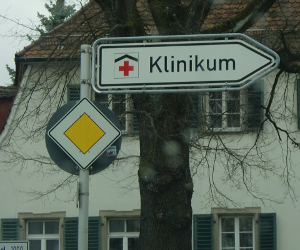
\includegraphics[width=0.3\textwidth]{plots/var_diff-klinikum_small.png} 
  }
  \subfigure[Test image 2]{
    \label{subfig:colorcheckerimg}
    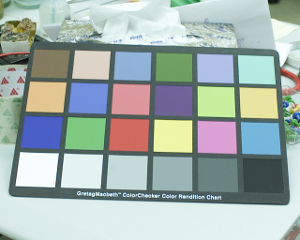
\includegraphics[width=0.3\textwidth]{plots/var_diff-colorchecker_small.png} 
  }
  \subfigure[Test image 3]{
    \label{subfig:stuffimg}
    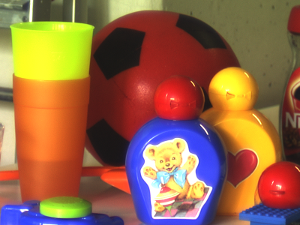
\includegraphics[width=0.3\textwidth]{plots/var_diff-stuff_small.png} 
  }
  \subfigure[$\beta$-map for \autoref{subfig:klinikumimg}]{
    \label{subfig:klinikum}
    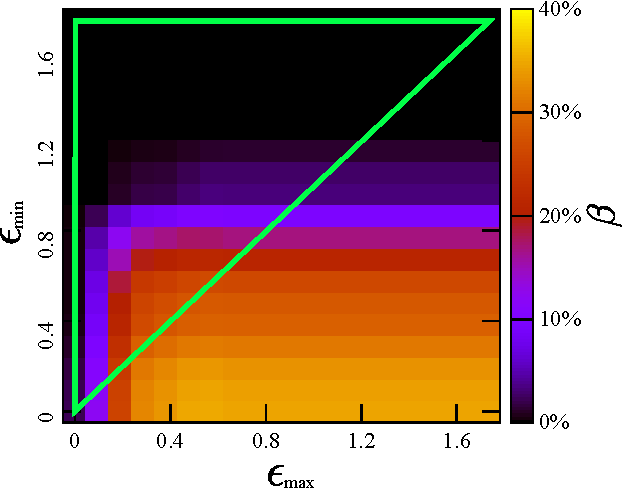
\includegraphics[width=0.31\textwidth]{plots/var_diff-klinikum.pdf} 
  }
  \subfigure[$\beta$-map for \autoref{subfig:colorcheckerimg}]{
    \label{subfig:colorchecker}
    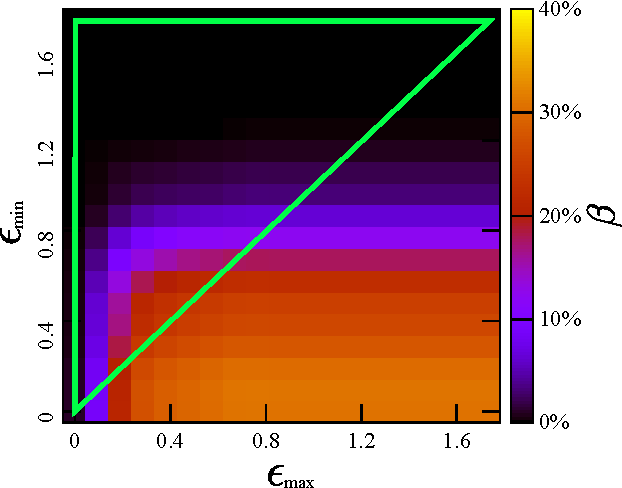
\includegraphics[width=0.31\textwidth]{plots/var_diff-colorchecker.pdf} 
  }
  \subfigure[$\beta$-map for \autoref{subfig:stuffimg}]{
    \label{subfig:stuff}
    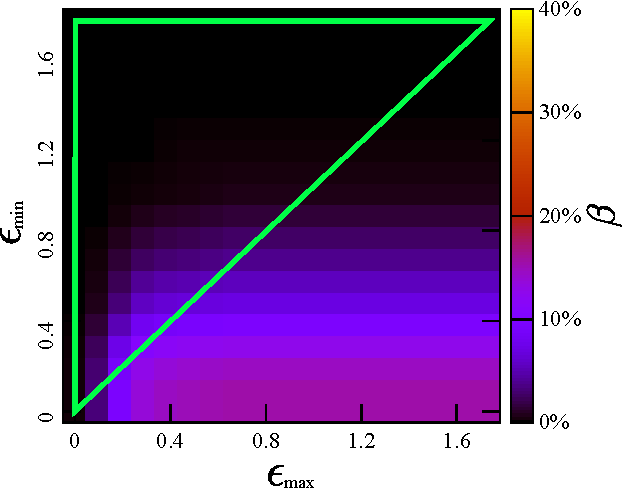
\includegraphics[width=0.31\textwidth]{plots/var_diff-stuff.pdf} 
  }
  \caption[Brute force determination of good values for $\epsilon_\text{min}$ and $\epsilon_\text{max}$]{Brute force determination of good values for $\epsilon_\text{min}$ and $\epsilon_\text{max}$. The first row contains the used images. The plot located below an image is its $\beta$-map, where brighter intensities (more yellow) represent higher color coverage. The green rectangle show the reasonable boundary for $\epsilon_\text{min}$ and $\epsilon_\text{max}$.}
  \label{fig:distanceparameterplots}
\end{figure}






\clearpage

\section{Tests with Synthetic Data}
\label{sec:syntheticdata}

\subsection{Experimental Setup}
\label{subsec:syntheticDataExperimentalSetting}

To examine the capabilities of the actual CRF estimation, a perfect observation set is assumed. The data acquisition step analyzed in the previous section is skipped and synthetic data is generated instead. A set of $N = 1500$ color triples ($C_1$, $C_2$, $C_{\text{edge}}$) is computed by picking the region colors $C_1$ and $C_2$ randomly for every color triple. Then, \autoref{eq:linearcombination} is used to get $C_{\text{edge}}$ with $\alpha = 0.5$. Now the situation is as in \autoref{subfig:irradiance}, an ideal CCD sensor is simulated. To emulate image intensity (\autoref{subfig:intensity}), a particular CRF $f$ is applied to all the colors in each color triple. In this chapter $f$ is a gamma curve with $\gamma \in \left\{0.2, 0.4, 0.6, 0.8, 1.0\right\}$. Note that ``more than $92 \%$ of the real-world digital camera CRFs in the DoRF database lie inbetween $r^{0.2}$ and $r^{0.6}$'' \cite{ng_cvpr07}. Hence, a linear gamma curve ($\gamma = 1.0$) is a quite unusual CRF.



\subsection{Error Measure}
\label{subsec:syntheticDataErrorMeasurement}

For the evaluation, an error function $\Psi(h_1, h_2)$ is introduced, which measures the dissimilarity of two distinct normalized two-dimensional functions $h_1$ and $h_2$.
\begin{equation}
	\Psi(h_1, h_2) = \frac{1}{M} \sum\limits_{i=1}^M \left( h_1\left(\frac{i}{M}\right) - h_2\left(\frac{i}{M}\right) \right)^2; \ \ M > 0 \enspace ,
	\label{eq:errfuncF1F2dissimilaritymeasure}
\end{equation}
where $M$ is the number of samples. For an illustration see \autoref{fig:errorfunctionPSI}. The left factor $1/M$ normalizes the error such that $\Psi \in \left[0;1\right]$, independent of $M$. The results in the following are obtained with $M = 1024$.
\begin{figure}[bt]
  \centering
  \subfigure[Example]{
    \label{subfig:exampleMeq6}
    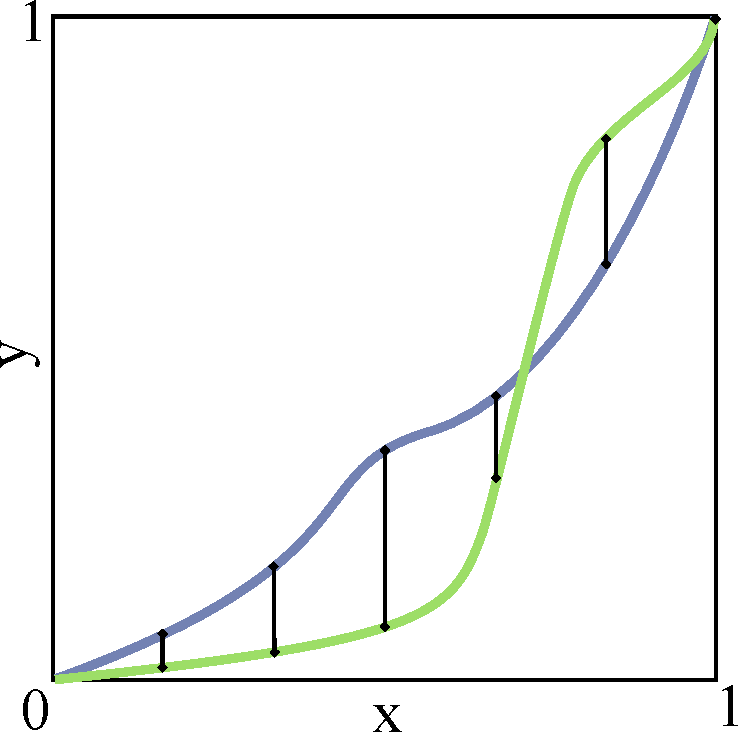
\includegraphics[width=0.3\textwidth]{images/error_function_psi_illustration.pdf} 
  }
  \subfigure[Example for maximum error]{
    \label{subfig:exampleMaxErr}
    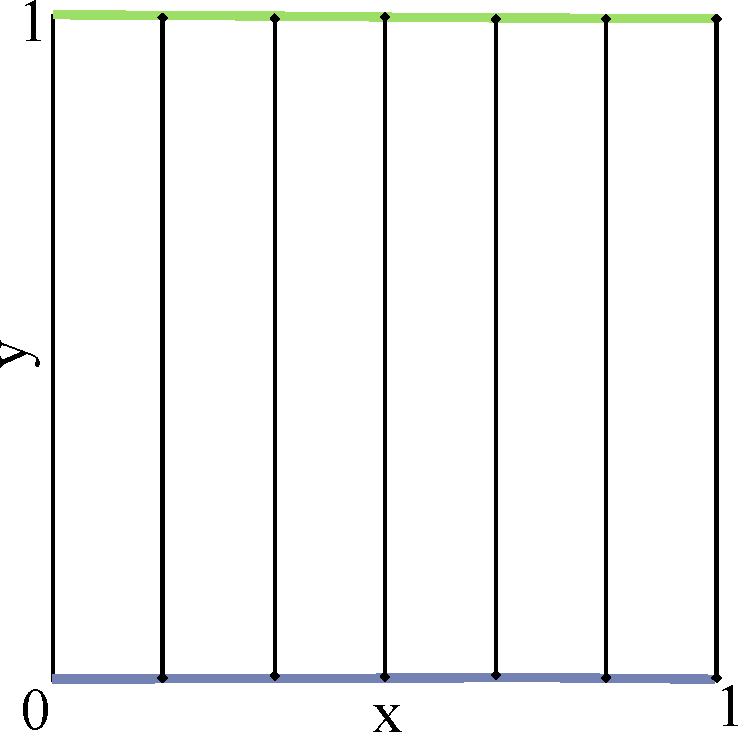
\includegraphics[width=0.3\textwidth]{images/error_function_psi_MAX_illustration.pdf} 
  }
  \caption[Error function illustration]{Error function illustration. $M$ is set to 6 for convenience. \autoref{subfig:exampleMeq6} shows two typical functions. The error is computed by adding up the length of the six black vertical lines squared each. The result is divided by $M$. An example which yields the maximum error function value is given in \autoref{subfig:exampleMaxErr} with $\Psi(h_1(x) = 0, h_2(x) = 1) = 1$.}
  \label{fig:errorfunctionPSI}
\end{figure}


\subsection{Results}
\label{subsec:syntheticDataResults}

In this section we will discuss the obtained results for four exemplary configurations of $(\kappa, \nu) \in \left\{ (3,3), (5,5), (5,7), (7,7) \right\}$. S. Lin, the author of \cite{Lin04radiometriccalibration}, proposed $\kappa = \nu = 5$, \hbox{i.e.} the number of kernels for the GMM $\kappa$ is set to 5, as well as the number of eigenvectors $\nu$ used for the PCA model.

The parameter $\lambda$ -- a weighting factor -- adjusts the impact of the \emph{prior model} based on the DoRF database versus the \emph{likelihood function}, which reflects the gathered data. For an explanation see \autoref{sec:radcal}. With increasingly large $\lambda$, more influence is passed to the information from the specific image (or from the image set). For very small $\lambda$, the estimated CRF is mainly based on the outcome of the EM algorithm, based on DoRF and controlled by $\kappa$ and $\nu$. 
\begin{figure}[tb]
	\centering
	\subfigure[$\kappa$ = 3; $\nu$ = 3]{
 	 \label{subfig:goodlambda3k3p}
 	 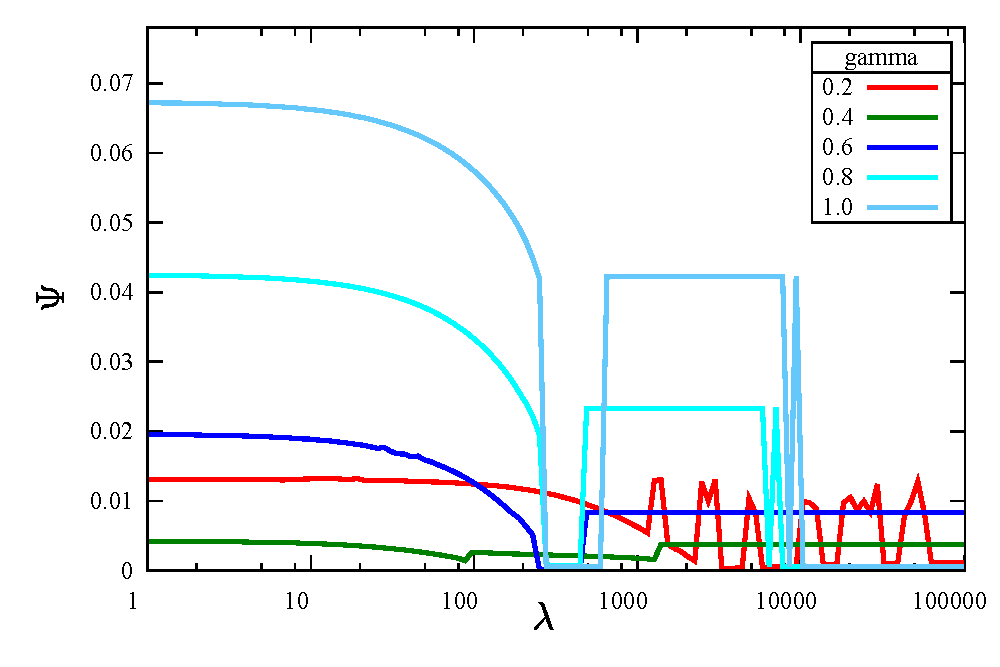
\includegraphics[width=0.483\textwidth]{plots/kernels3components3.pdf} 
  }
	\subfigure[$\kappa$ = 5; $\nu$ = 5]{
 	 \label{subfig:goodlambda5k5p}
 	 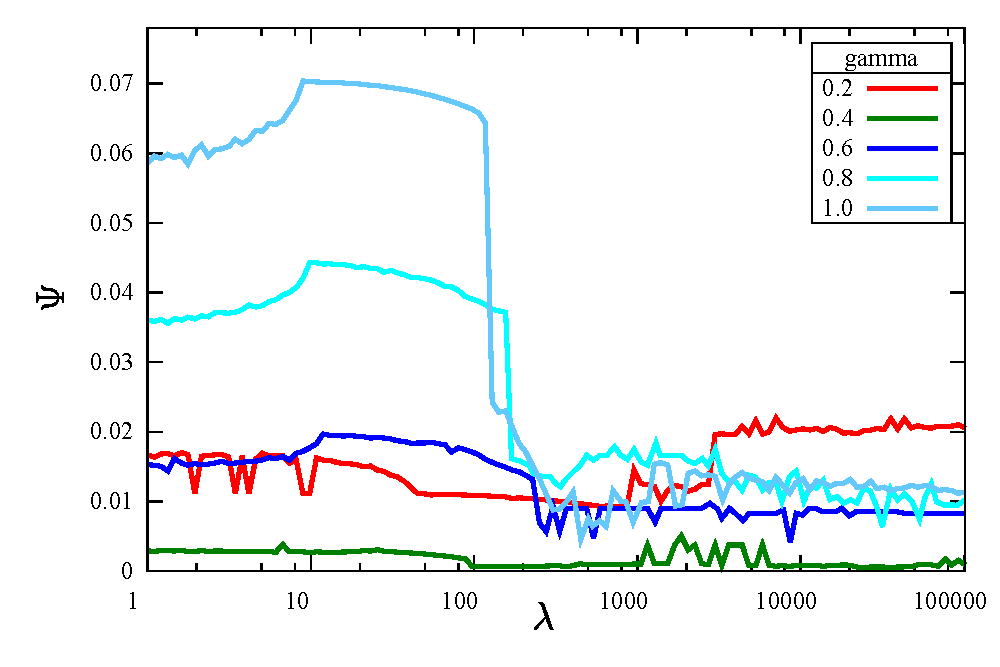
\includegraphics[width=0.483\textwidth]{plots/kernels5components5.pdf} 
  }
  \subfigure[$\kappa$ = 5; $\nu$ = 7]{
 	 \label{subfig:goodlambda5k7p}
 	 \includegraphics[width=0.483\textwidth]{plots/kernels5components7.pdf} 
  }
  \subfigure[$\kappa$ = 7; $\nu$ = 7]{
 	 \label{subfig:goodlambda7k7p}
 	 \includegraphics[width=0.483\textwidth]{plots/kernels7components7.pdf} 
  }
  \caption[Determination of balanced value for $\lambda$]{Determination of balanced value for $\lambda$. The error measurements $\Psi$ of the estimated curve to the ground-truth inverse CRF are visualized for four different configurations of $(\kappa, \nu)$ and five different gamma curves each. The presented curves interpolate between more than 120 logarithmic distributed measurements per gamma curve.}
	\label{fig:goodlambda}
\end{figure}

Considering perfect conditions as is the case with the above presented synthetic data, a very large value of $\lambda$ might be preferred. This means, that the examined image exhibits many distinct but uniform regions with almost no noise and thus the observation set is very well compiled, \hbox{e.g.} the color coverage factor $\beta$ reaches almost $100 \%$. 

Note that not even with $\lambda \rightarrow \infty$ the method is highly influenced by the ground-truth (\hbox{i.e.} $\Psi \rightarrow 0$) for many CRFs, because the optimization step -- starting from the DoRF mean curve $g_\text{DoRF}$ -- is still very much dependent on the PCA representation of the inverse CRF, which again is based on DoRF. So for this method, prior knowledge can not be \emph{switched off} and thus it is not a good choice if the examined images are taken by cameras with very unusual CRFs like a linear curve (in case of gamma curves: $\gamma = 1.0$).

Interpretation approaches for observations, which the results for all examined parameter setups have in common, are presented in the following on page \pageref{subsubsec:commonobservations}. This is continued by setup-specific observations. The actual results are shown in \autoref{fig:goodlambda}. Note the log scale on the horizontal axis ($\lambda$).



\clearpage

\subsubsection{Common Observations for all Settings}
\label{subsubsec:commonobservations}

For all parameter settings in \autoref{fig:goodlambda}, the (quite) linear CRFs ($\gamma = 1.0$ and $\gamma = 0.8$) have at least for $1 \leq \lambda \leq 200$ a very high error, \hbox{i.e.} the estimated function and the ground-truth are quite dissimilar. The reason is that they differ the most from $g_\text{DoRF}$. In contrast, the error measurements presented in green ($\gamma = 0.4$) consistently exhibit a very small error. Hence, $g_\text{DoRF}$ must be most similar to a gamma curve with $\gamma = 0.4$. Therefore, the measured values are mostly below $\Psi < 0.005$ for nearly any value of $\lambda$.

The trend of the red curve, representing the error measurements for a gamma curve with $\gamma = 0.2$, differs from the others. Except for the measurements in \autoref{subfig:goodlambda3k3p}, $\Psi$ does not get significantly smaller by increasing $\lambda$. In \autoref{subfig:goodlambda5k5p}, $\Psi$ even increases. Here, $\Psi$ for $\lambda = 10000$ is about $90\%$ larger than for $\lambda = 500$. Starting from a particular $\lambda$, even the quite unusual CRF, the linear curve ($\gamma = 1.0$), outperforms this gamma curve. We can not explain this phenomenon so far. 

For fixed $\nu$, but varying number of kernels for the Gaussian mixture model $\kappa$, an interesting observation can be extracted by comparing \autoref{subfig:goodlambda5k7p} to \autoref{subfig:goodlambda7k7p}. The two plots do not differ very much. Indeed, \autoref{subfig:goodlambda7k7p} looks like a smoothed version of \autoref{subfig:goodlambda5k7p}. Although the presumable expectation would be, that $\Psi$ varies more for a larger number of kernels than for smaller $\kappa$, the opposite is observed.



\subsubsection{Parameter-specific Observations}
\label{subsubsec:paramspecificobservations}

The error for small $\lambda$ is much larger for the settings presented in the first row than for those in the second row. We observed, that the number of used eigenvectors $\nu$ has significant impact on the shape of the estimated inverse CRF, what could be a reason for this effect.

In \autoref{subfig:goodlambda3k3p}, the trends of the blue curves ($\gamma \in \left\{0.8, 1.0\right\}$) exhibit significant unexpected changes. Around $\lambda \approx 800$, the previously decreasing or very low error measurements turn into horizontal lines until $\lambda \approx 10000$. A possible explanation for this effect is, that the LM minimization converges at a local minimum for several consecutive values of $\lambda$.

Regarding the curves with $\gamma \in \left\{0.6, 0.8, 1.0\right\}$ in \autoref{subfig:goodlambda5k5p}, another interesting aspect is the at first monotonically increasing error function values until $\lambda \approx 12$, where $\Psi$ suddenly decreases. A possible explanation for this effect is given by example. The prior model is a Gaussian mixture model with $\kappa$ kernels. A (inverse) CRF is represented by a $\nu$-dimensional vector. Without loss of generality, let $\nu = 2$ and $\kappa = 4$. So there is a two-dimensional space with four two-dimensional Gaussian bells. The ground-truth curve and the estimated curve are referred to as $\vec{p}_{\text{gt}}$ and $\vec{p}_{\text{est}}$. For a very small $\lambda = 1$, $\vec{p}_{\text{est}}$ is near the point representing the mean curve $\vec{p}_{\text{mean}}$. With increasing $\lambda$, the influence of the prior knowledge slowly decreases and thus $\vec{p}_{\text{est}}$ starts drifting towards the ground-truth $\vec{p}_{\text{gt}}$. But on the path from $\vec{p}_{\text{mean}}$ to $\vec{p}_{\text{gt}}$ some \emph{hurdles} (the Gaussian kernels) have to be passed, which -- if the influence of the prior model is still too high -- can \emph{pull} $\vec{p}_{\text{est}}$ into the wrong direction temporarily. But starting from a specific $\lambda \approx 12$, the \emph{pulling capabilities} of the kernels are not sufficient anymore and $\vec{p}_{\text{est}}$ continues traveling into the direction of its desired destination $\vec{p}_{\text{gt}}$. This process is outlined in \autoref{fig:lambdapath}. The image can be seen as an excerpt of the two-dimensional (inverse) CRF space using the PCA representation. Note that the distance between $\vec{p}_{\text{est}}$ and $\vec{p}_{\text{gt}}$ slightly increases for small $\lambda$ as pointed out above.

\begin{figure}[tb]
	\centering
		\includegraphics[width=0.5\textwidth]{images/lambda_path.png}
	\caption[Sketch of $\lambda$ influence]{Sketch of $\lambda$ influence. The red star depicts $\vec{p}_{\text{mean}}$ and the green star $\vec{p}_{\text{gt}}$. The dotted white line sketches the path of $\vec{p}_{\text{est}}$, when $\lambda$ is increasing. An exemplary GMM obtained by the EM algorithm is visualized by the underlying map.}
	\label{fig:lambdapath}
\end{figure}






\clearpage

\section{Stability Tests}
\label{sec:stability}

Purposely, neither the approach from \autoref{sec:capabilitiesofdataacqu} nor the one from \autoref{sec:syntheticdata} covered the whole algorithm as presented in \autoref{subsec:radcalalgo}. The two main steps, the observation set formation and the optimization step, were treated separately -- independently from each other -- to find reliable settings for the most significant parameters. Hence, the goal of this part of the thesis is to evaluate the method considering the \emph{entire} procedure, while using the previously obtained knowledge on the crucial parameters. 


\subsection{Prerequisites}
\label{subsec:stabilityPrerequisites}

A commonly used approach is to assess the robustness of a method. Therefore 8 sets of images from 8 different cameras were compiled with an average of about 50 images per camera. Only images with a very high probability not being post-processed in image manipulation tools like ``Adobe Photoshop'' \cite{photoshop} or ``GIMP, The GNU Image Manipulation Program'' \cite{gimp} were taken into the sets. The reason is that such software can manipulate images in a way, that an estimation of the actually applied CRF gets impossible. Therefore the collected photos were either
\begin{itemize}
	\item photographs from our own cameras, which are certainly in their original state or
	\item amateur shots from online resources like \emph{picasaweb}\footnote{\url{http://picasaweb.google.com/}} or \emph{flickr}\footnote{\url{http://www.flickr.com/}} tagged ``not manipulated'' or similarly.
\end{itemize}
Many prestigious camera manufacturers are covered: Canon, Sony, Casio, FujiFilm and two camera models each from Kodak and Nikon. Both professional camera models like the Canon EOS 400D Rebel XTi and cheaper models for beginners like the Casio Exilim EX-S600 are examined. 

We also included about 250 samples from a publicly available database of RGB color images \cite{ciurea2003large} in our tests. It consists of 11000 images and is primarily intended for color constancy research. The assumption is, that for each image in the database, the CRF is approximately similar. Hence, we can test the robustness of the examined method for this set of images, too. This database is referred to as ``Funt database'' in the following. Due to the fact, that the images in this database are relatively small sized ($360 \times 240$ pixels), the size of the patches was decreased to $W = H = 12$ and thus also the maximum dilation distance is set to $2$.



\subsection{Leave-One-Out Approach}
\label{subsec:stabilityLOO}

As the name suggests, the leave-one-out (LOO) technique uses only a single observation -- in this case only one estimated inverse CRF from a whole set of inverse CRFs -- per iteration to obtain error measurements. The successive steps for this evaluation approach are described in the following, while a simplified visualization of the functional principle is presented in \autoref{fig:leaveOneOut}.

\begin{figure}[tb]
	\centering
	\includegraphics[width=0.8\textwidth]{images/loo_description.pdf}
	\caption[Leave-one-out overview]{Leave-one-out overview. This figure represents a simplified version, where only one channel is shown. Note that the error is measured between the \emph{left out} curve and the mean curve computed over the \emph{other} curves.}
	\label{fig:leaveOneOut}	
\end{figure}

Given a set of $n$ images taken with the same camera, the algorithm as presented in \autoref{subsec:radcalalgo} is conducted on each image seperately. This produces a set $\mathcal{G}$ of $n$ inverse CRF triples 
\begin{equation}
	\mathcal{G} = \left\{\vec{g}_i = 
	\begin{pmatrix} g_{i_\text{red}} \\ g_{i_\text{green}} \\ g_{i_\text{blue}} \end{pmatrix}; \ i=1 \ldots n\right\} \enspace ,
	\label{eq:setOfInverseCRFs}
\end{equation}
where for each image three inverse CRFs -- one for each channel (red, green and blue) -- are estimated, \hbox{i.e.} altogether $3n$ inverse camera response function.

Now a set $\mathcal{E}$ of three-dimensional error vectors $\vec{e}_i \in \mathcal{E}$ is obtained by evaluating
\begin{equation}
	\vec{e}_i = 
	\begin{pmatrix}
		e_{i_\text{red}}   &=& \Psi \left( g_{i_\text{red}}, \mathrm{mean} \left( \mathcal{G}_\text{red} \setminus \left\{ g_{i_\text{red}} \right\} \right) \right) \\
		e_{i_\text{green}} &=& \Psi \left( g_{i_\text{green}}, \mathrm{mean} \left( \mathcal{G}_\text{green} \setminus \left\{ g_{i_\text{green}} \right\} \right) \right) \\
		e_{i_\text{blue}}  &=& \Psi \left( g_{i_\text{blue}}, \mathrm{mean} \left( \mathcal{G}_\text{blue} \setminus \left\{ g_{i_\text{blue}} \right\} \right) \right)
	\end{pmatrix}
	\label{eq:errorVector}
\end{equation}
for each $\vec{g}_i \in \mathcal{G}$. $\mathcal{G}_c$ is the set of inverse CRFs for a particular channel $c \in \{\text{red}, \text{green}, \text{blue}\}$ extracted from $\mathcal{G}$. $\Psi$ is the error measurement from \autoref{eq:errfuncF1F2dissimilaritymeasure} and the function $\mathrm{mean}$ computes the mean curve of the given set of inverse CRFs. The best and worst case for each channel, \hbox{i.e.} the minimum error $e_\text{min}$ and maximum error $e_\text{max}$ are stored.

In the next step the mean error $\mu_c$ per channel $c$ is computed by 
\begin{equation}
	\mu_c = \frac{1}{n} \sum\limits_{i=1}^{n} e_{i_c} \enspace .
	\label{eq:meanErrorComputationPerChannel}
\end{equation}

Besides the mean error $\mu$, its standard deviation $\sigma$ is also a meaningful measurement. Therefore, $\sigma_c$ is obtained for each channel $c$ by
\begin{equation}
	\sigma_c = \sqrt{\sigma_c^2} = \sqrt{ \frac{1}{n} \sum\limits_{i=1}^{n} \left( e_{i_c} - \mu_c \right)^2 } \enspace .
	\label{eq:stddev}
\end{equation}

To get an overall measurement, \hbox{i.e.} for the entire camera and thus for all three channels combined, the joint mean error $\mu_\text{joint}$ and the joint standard deviation $\sigma_\text{joint}$ for all channels is computed as well.
\begin{eqnarray}
	\mu_\text{joint}    &=& \frac{1}{3 n} \sum\limits_{i=1}^{n} \left( e_{i_\text{red}} + e_{i_\text{green}} + e_{i_\text{blue}} \right) \enspace \text{and} \\
	\label{eq:meanErrorJoint}
	\sigma_\text{joint} &=& \sqrt{ \frac{1}{3 n} \sum\limits_{i=1}^{n} \left( \left( e_{i_\text{red}} - \mu_\text{joint} \right)^2 + \left( e_{i_\text{green}} - \mu_\text{joint} \right)^2 + \left( e_{i_\text{blue}} - \mu_\text{joint} \right)^2 \right) } \enspace .
	\label{eq:StdDevJoint}
\end{eqnarray}


\clearpage

\subsection{Results}
\label{subsec:stabilityResults}

Our results presented in this section were obtained using different parameter setups for $\kappa$, $\nu$ and $\lambda$. The main quality factor is the joint mean error $\mu_\text{joint}$, \hbox{i.e.} the smaller $\mu_\text{joint}$ is, the more robust is the method for a particular set of images. For these tests, images with a color coverage factor $\beta < 5\%$ were ignored. 

The examination of the parameter $\lambda$ in \autoref{sec:syntheticdata} leads to the assumption, that the robustness for small $\lambda$ is better than for big $\lambda$. The reason is the merely minor impact of the image-specific information for small $\lambda$. Hence, the estimation is mainly affected by the prior model, which is equal for every image. Consequently, the resulting inverse CRFs will not differ a lot and thus $\mu_\text{joint}$ will be significantly lower than for large $\lambda$. Note that a small $\mu_\text{joint}$ does not necessarily implicate good estimates in comparison to the unknown ground-truth inverse CRF.

\autoref{fig:lambdavariation} illustrates the increasing value for $\mu_\text{joint}$ for increasing $\lambda$. The two cameras Canon EOS 400D and Sony CyberShot DSC-W300 are compared directly. For all three presented configurations of $(\kappa, \nu) \in \left\{(3,3), (5,5), (7,7)\right\}$, the inequation $\mu_\text{joint}(100) < \mu_\text{joint}(1000) < \mu_\text{joint}(10000)$ holds. The only exception is for the Funt database. There, for the settings $(\kappa,\nu) \in \left\{ (3,3), (5,5) \right\}$, $\mu_\text{joint}(10000) < \mu_\text{joint}(1000)$.
\begin{figure}[btp]
  \centering
	 \subfigure[Canon EOS 400D -- $\kappa$ = 3; $\nu$ = 3]{
 	 \label{subfig:canoneos3k3c_lambda_diff}
 	 \includegraphics[width=0.4\textwidth]{plots/canoneos3k3c_lambda_diff.pdf}
  }
  \subfigure[Sony CyberShot DSC-W300 -- $\kappa$ = 3; $\nu$ = 3]{
    \label{subfig:sony3k3c_lambda_diff}
    \includegraphics[width=0.4\textwidth]{plots/sony3k3c_lambda_diff.pdf}
  }
  \subfigure[Canon EOS 400D -- $\kappa$ = 5; $\nu$ = 5]{
 	 \label{subfig:canoneos5k5c_lambda_diff}
 	 \includegraphics[width=0.4\textwidth]{plots/canoneos5k5c_lambda_diff.pdf}
  }
  \subfigure[Sony CyberShot DSC-W300 -- $\kappa$ = 5; $\nu$ = 5]{
    \label{subfig:sony5k5c_lambda_diff}
    \includegraphics[width=0.4\textwidth]{plots/sony5k5c_lambda_diff.pdf}
  }
  \subfigure[Canon EOS 400D -- $\kappa$ = 7; $\nu$ = 7]{
 	 \label{subfig:canoneos7k7c_lambda_diff}
 	 \includegraphics[width=0.4\textwidth]{plots/canoneos7k7c_lambda_diff.pdf}
  }
  \subfigure[Sony CyberShot DSC-W300 -- $\kappa$ = 7; $\nu$ = 7]{
    \label{subfig:sony7k7c_lambda_diff}
    \includegraphics[width=0.4\textwidth]{plots/sony7k7c_lambda_diff.pdf}
  }
  \caption[Increasing $\mu_\text{joint}$ for increasing $\lambda$]{Increasing $\mu_\text{joint}$ for increasing $\lambda$. The red bars show the actual measurements and their standard deviations $\sigma_\text{joint}$. The green curve interpolates between the measurements. In each row, $\kappa$ and $\nu$ are fixed. Note the log scale on the horizontal axis.}
  \label{fig:lambdavariation}
\end{figure}

The overall best result in terms of robustness is presented in \autoref{tab:Canon EOS 400D Rebel XTi77100 - inText}. The first three columns represent the red, green and blue channel. In the last two rows of the fourth column, the two measurements from \autoref{eq:meanErrorJoint} are located. The most meaningful measurement $\mu_\text{joint}$ is printed in bold. Note the relatively small value of $\lambda = 100$. It is actually the smallest one used for this evaluation approach. Hence, the previously made assumption on $\lambda$ turned out to be true for our experiments. 

The worst observation, \hbox{i.e.} the largest value for $\mu_\text{joint}$, was observed for the highest used value of $\lambda = 10000$. It is presented in \autoref{tab:Kodak DX75903310000 - inText}. The mean joint error is about 200 times larger in comparison to the best case.
\begin{table}[tb]
  \centering
    \begin{tabular}{|c||c|c|c|c|}\hline
		   & \textbf{Red} & \textbf{Green} & \textbf{Blue} & \textbf{$\sum$} \\\hline\hline
      $e_\text{min}$ & 0.000053 & 0.000053 & 0.000053 &   \\\hline
      $e_\text{max}$ & 0.000363 & 0.000512 & 0.000605 &   \\\hline
      $\mu$          & 0.000079 & 0.000076 & 0.000087 & \textbf{0.000081} \\\hline
      $\sigma$       & 0.000019 & 0.000018 & 0.000029 & 0.000022 \\\hline
    \end{tabular}
  \caption{Best stability: Canon EOS 400D -- $\kappa$ = 7; $\nu$ = 7; $\lambda$ = 100}
  \label{tab:Canon EOS 400D Rebel XTi77100 - inText}
\end{table}
\begin{table}
  \centering
    \begin{tabular}{|c||c|c|c|c|}\hline
		   & \textbf{Red} & \textbf{Green} & \textbf{Blue} & \textbf{$\sum$} \\\hline\hline
      $e_\text{min}$ & 0.004425 & 0.002074 & 0.002261 &   \\\hline
      $e_\text{max}$ & 0.158236 & 0.085810 & 0.064222 &   \\\hline
      $\mu$          & 0.017749 & 0.015236 & 0.015869 & \textbf{0.016285} \\\hline
      $\sigma$       & 0.017430 & 0.013811 & 0.013130 & 0.014790 \\\hline
    \end{tabular}
  \caption{Worst stability: Kodak DX7590 -- $\kappa$ = 3; $\nu$ = 3; $\lambda$ = 10000}
  \label{tab:Kodak DX75903310000 - inText}
\end{table}

Some of the actually estimated inverse CRFs for the best and worst results as well as for an average case and some examples of the Funt database are presented in \autoref{fig:samplecurvesStability}. The effects of having good or bad robustness, \hbox{i.e.} small or large values of $\mu_\text{joint}$, can obviously be observed in these plots. In \autoref{fig:meancurvesred}, the \emph{mean} inverse CRFs for the best and the worst result are shown. They are both very similar to the DoRF mean curve.

\begin{figure}[bt]
  \centering
  \subfigure[Canon EOS 400D -- $\kappa$ = 7; $\nu$ = 7; $\lambda$ = 100]{
 	 \label{subfig:bestSampleCurves}
 	 \includegraphics[width=0.4\textwidth]{plots/best_sample_curves.pdf}
  }
  \subfigure[Kodak DX7590 -- $\kappa$ = 3; $\nu$ = 3; $\lambda$ = 10000]{
 	 \label{subfig:worstSampleCurves}
 	 \includegraphics[width=0.4\textwidth]{plots/worst_sample_curves.pdf}
  }
  \subfigure[Nikon D40 -- $\kappa$ = 5; $\nu$ = 5; $\lambda$ = 10000]{
 	 \label{subfig:avgSampleCurves}
 	 \includegraphics[width=0.4\textwidth]{plots/average_sample_curves.pdf}
  }
  \subfigure[Funt database -- $\kappa$ = 7; $\nu$ = 7; $\lambda$ = 10000]{
 	 \label{subfig:funtSampleCurves}
 	 \includegraphics[width=0.4\textwidth]{plots/funt_sample_curves.pdf}
  }
  \caption[Sample inverse CRF estimates (stability test)]{Sample inverse CRF estimates for the best (\autoref{subfig:bestSampleCurves}) and the worst (\autoref{subfig:worstSampleCurves}) stability. Samples for an average value of $\mu_\text{joint}$ are presented in \autoref{subfig:avgSampleCurves} and representative estimates from the Funt database in \autoref{subfig:funtSampleCurves}.}
  \label{fig:samplecurvesStability}
\end{figure}

\begin{figure}[bt]
	\centering
 	\includegraphics[width=0.35\textwidth]{plots/best_vs_worst_mean_red_channel.pdf}
	\caption[Best and worst mean curve]{Mean curves for best (green) and worst (red) stability (for the red channel). The dotted curve represents the mean inverse CRF from DoRF.}
\label{fig:meancurvesred}	
\end{figure}

To get an overall impression of the obtained results, we created a plot of all tested datasets and parameters (see \autoref{fig:bigcomparison}). It reflects the previously made conclusions. Note that the figure is subdivided into three distinct plots, one for each configuration of $(\kappa, \nu)$, illustrated by the dashed vertical lines. The horizontal axis differentiates the values of $\lambda$ and the vertical axis shows the error measure $\mu_\text{joint}$. The most stable results, independently of the chosen parameters, are obtained for the set of images from Canon EOS 400D and from the Funt database. Some sample estimated inverse CRFs from the Funt database are shown in \autoref{subfig:funtSampleCurves}. 

It turned out, that if only small values for $\kappa$ and $\nu$ are chosen, \hbox{e.g.} $(3,3)$, worse stability is measured than for larger values. Furthermore, the best results in terms of both, stability and similarity to the ground-truth curve combined, are the results with the smallest values of $\mu_\text{joint}$ for the largest value of $\lambda = 10000$. The reason is, that even though the prior model has only little impact on the estimates, the algorithm returns quite similar inverse CRFs. Hence, the image-specific observation set seems to be rather well compiled and also the CRF estimation step produced good results. All in all, the entire algorithm reached rather good performance.

Some additional tables for two different parameter setups are presented in \autoref{chap:additionalTables}.

\begin{figure}[bt]
	\centering
 	\includegraphics[width=0.95\textwidth]{stabilitytest/big_comparison.pdf}
	\caption[Overview of all obtained results]{Overview of all obtained results. The dotted curves connect the consecutive measurements of the same camera.}
\label{fig:bigcomparison}	
\end{figure}   % (\chapter{})
\cleardoublepage
\chapter{Summary \& Outlook}
\label{chap:summaryoutlook}

Todays digital cameras apply a large amount of post-processing on a captured image. Typically, this post-processing aims at creating more visually pleasing, crisp and clean images. Many of these steps are nonlinear, like for instance white balancing to compensate for different light temperature or gamma correction. All these nonlinearities can be summarized as a single function, the camera response function (CRF). However, many algorithms in computer vision require images, where the intensities are approximately linear to the real-world scene radiance. Prominent examples for such algorithms are \emph{Color Constancy} or \emph{Shape from Shading}. Digital cameras are available, of which the direct output of the CCD sensor can be extracted, which is supposed to be linear. Nevertheless, to be able to conduct these algorithms on arbitrary images from all kinds of sources, methods were developed to estimate the CRF of a particular camera. Knowing the CRF facilitates mapping image intensity back to approximately linear image irradiance by inverting the CRF. Recently, several approaches on this topic have been proposed. Most of them require several images taken in constrained environments and thus they can not be applied on arbitrary images.

In this thesis, two approaches on the estimation of the CRF from a single RGB color image are examined. The approach by Ng et \hbox{al.}, ``Using Geometry Invariants for Camera Response Function Estimation'', is physics-based. Locally planar irradiance points (LPIPs) are used to extract information solely related to the particular CRF. If a point has an irradiance geometry that is locally planar, then the second order partial derivatives in the irradiance domain would all be zero. Consequently, an equation called \emph{derivative equality constraint} holds, which is referred to as first order geometry invariant ($G_1$). This quantity does not carry any geometry information and thus is used to estimate the CRF. Therefore, it is shown that $G_1$ has a simple relationship with the gamma curve parameter $\gamma$. A related expression is introduced ($Q(R)$). The subsequent steps are first, extracting LPIPs from an image and computing $G_1$. Then the extracted points get weighted utilizing $Q(R)$ in combination with Bayesian inference to overcome problems with erroneously detected points. The third step is done by an iterative minimization algorithm. It looks for the optimal parameters for a specific CRF model. The utilized model is called generalized gamma curve model (GGCM). Ng et \hbox{al.} introduced this extension to the pure gamma curve model, because it has quite good fit to real-world CRFs in comparison to more conventional models.

Despite thorough studies, including spending much effort on locating potential error sources, we could not achieve satisfying results. The problem first appears when computing $Q(R)$. Due to the fact that $Q(R)$ is strongly related to the applied CRF, histograms are generated, which can be interpreted to estimate the CRF. However, the expected CRF-dependent distribution of the $Q(R)$-values could not be observed. It turned out, that we were not able to successfully perform Bayesian inference on our version of the $Q$-$R$-histograms. Nevertheless, an approach for further examination of this method is proposed.

The second method, proposed by S. Lin et \hbox{al.}, ``Radiometric Calibration from a Single Image'', utilizes the nonlinear edge color distributions emerging by applying a nonlinear CRF. It is shown that the colors on an edge between two distinct regions, which are both colored uniformly, result in a linear combination of the two region colors in scene irradiance. Hence, the edge colors lie on the line spanned by the two region colors in RGB space. After the nonlinear CRF transformation, the edge colors are located on a curve rather than a line. This fact is used to estimate the CRF. For reasons of interpolating over regions of only sparse color coverage, and to overcome very unstable estimates occurring due to the presence of noise, prior knowledge on CRFs is involved. A PCA representation of CRFs is utilized to model the space of characteristic real-world CRFs. Therefore, the CRF space is modeled by a Gaussian mixture model (GMM) of real-world CRFs. The algorithm is subdivided into two main steps. At first, image-specific information is collected by looking for patches of a certain size, containing exactly one edge and two distinct color regions. An observation set is formed. Secondly, the CRF is estimated by incorporating both, the prior model and the image-specific information. The Levenberg-Marquardt minimization routine is used for optimization.

We evaluated the two main steps of this method. At first, both steps are discussed separately, independently from each other, assuming perfect conditions. The goal was to examine how well the method can perform in theory and to determine a set of good parameters for the final evaluation, a stability test.

During the evaluation of the data acquisition step, it turned out, that two parameters mainly determine the quality and size of the resulting observation set. Besides the size of the set, also its coverage of the color space used by the examined image is important. We introduced an algorithm to measure a quantity called color coverage factor $\beta$. Incorporating $\beta$, a brute force approach facilitated finding a good combination of these two most significant parameters.

The second evaluation approach aims at the maximum possible performance of the CRF estimation step. For this purpose, the data acquisition step is skipped and perfect, synthetic data without noise is generated instead. Note that due to the data being synthetically generated, the ground-truth CRF is known. The most influential parameter here is $\lambda$. It balances the impact of image-specific information versus prior knowledge. The most important insight is, that the error of the estimated CRF to the ground-truth CRF can be significantly decreased, when additional knowledge on the type of the CRF is available. This means, that if the CRF is a typical one, then the impact of the prior knowledge should be greater than for very uncommon CRFs, like linear ones. The reason is, that even very noisy and corrupt data in the observation set can not significantly lower the quality of the estimates, if prior knowledge is highly weighted. Vice versa, having a linear CRF, most influence should be passed to the image-specific information. Otherwise, the estimates will remain relatively similar to typical CRFs.

In the final evaluation, we combined both previously examined steps and examined real-world images. Sets of same-camera natural images were compiled to measure the robustness of this method utilizing a leave-one-out (LOO) approach. The main quality criterion determining the actual robustness is the mean error over all three color channels and the standard deviation of the error measurements. It turned out, that the stability of the method is heavily dependent on the chosen parameters, in particular $\lambda$. As expected, if the prior knowledge is weighted more strongly, the method is much more robust. But this does not necessarily imply, that the estimated CRFs are more similar to the ground-truth curves. Only the dissimilarity between a set of CRFs computed from images taken by the same camera is smaller. We compared eight different cameras from prestigious manufacturers. Also an image database, rather intended for color constancy research, is involved. For this set of images, some differences to those from the other cameras were observed. A possible explanation is, that this database is extracted from a video camera, while all the other cameras are usual digital cameras.

All in all, modern digital cameras change the actually measured scene radiance in a vast number of ways. New camera generations have new features, that make the images look more impressive. Therefore, CRF estimation will be challenging the computer vision community for a long time.   % (\chapter{})
\cleardoublepage
\begin{appendix}
%\chapter{Additional Figures}
%\label{chap:additionalFigures}
%
%
%\cleardoublepage
%
\chapter{Additional Tables}
\label{chap:additionalTables}
\begin{table}[htb]
  \centering
    \begin{tabular}{|c||c|c|c|c|}\hline
		   & \textbf{Red} & \textbf{Green} & \textbf{Blue} & \textbf{$\sum$} \\\hline\hline
      $e_\text{min}$ & 0.000041 & 0.000037 & 0.000051 &   \\\hline
      $e_\text{max}$ & 0.005552 & 0.005334 & 0.028683 &   \\\hline
      $\mu$          & 0.001451 & 0.001259 & 0.002995 & \textbf{0.001902} \\\hline
      $\sigma$       & 0.001167 & 0.001115 & 0.003327 & 0.001869 \\\hline
    \end{tabular}
  \caption{Canon EOS 400D Rebel XTi -- $\kappa$ = 5; $\nu$ = 5; $\lambda$ = 1000}
  \label{tab:Canon EOS 400D Rebel XTi551000}
\end{table}
\begin{table}[htb]
  \centering
    \begin{tabular}{|c||c|c|c|c|}\hline
		   & \textbf{Red} & \textbf{Green} & \textbf{Blue} & \textbf{$\sum$} \\\hline\hline
      $e_\text{min}$ & 0.000425 & 0.000625 & 0.001365 &   \\\hline
      $e_\text{max}$ & 0.009518 & 0.007175 & 0.026447 &   \\\hline
      $\mu$          & 0.003796 & 0.003014 & 0.008503 & \textbf{0.005104} \\\hline
      $\sigma$       & 0.003121 & 0.002270 & 0.007144 & 0.004178 \\\hline
    \end{tabular}
  \caption{Casio Exilim EX-S600 -- $\kappa$ = 5; $\nu$ = 5; $\lambda$ = 1000}
  \label{tab:Casio Exilim EX-S600551000}
\end{table}
\begin{table}[htb]
  \centering
    \begin{tabular}{|c||c|c|c|c|}\hline
		   & \textbf{Red} & \textbf{Green} & \textbf{Blue} & \textbf{$\sum$} \\\hline\hline
      $e_\text{min}$ & 0.000521 & 0.000774 & 0.000071 &   \\\hline
      $e_\text{max}$ & 0.031596 & 0.011812 & 0.028996 &   \\\hline
      $\mu$          & 0.005836 & 0.005034 & 0.006148 & \textbf{0.005673} \\\hline
      $\sigma$       & 0.005431 & 0.003518 & 0.005009 & 0.004653 \\\hline
    \end{tabular}
  \caption{FujiFilm FinePix S5600 -- $\kappa$ = 5; $\nu$ = 5; $\lambda$ = 1000}
  \label{tab:FujiFilm FinePix S5600551000}
\end{table}
\begin{table}[htb]
  \centering
    \begin{tabular}{|c||c|c|c|c|}\hline
		   & \textbf{Red} & \textbf{Green} & \textbf{Blue} & \textbf{$\sum$} \\\hline\hline
      $e_\text{min}$ & 0.000302 & 0.000234 & 0.000150 &   \\\hline
      $e_\text{max}$ & 0.049095 & 0.065609 & 0.031550 &   \\\hline
      $\mu$          & 0.007401 & 0.005136 & 0.006189 & \textbf{0.006242} \\\hline
      $\sigma$       & 0.006646 & 0.004835 & 0.004863 & 0.005448 \\\hline
    \end{tabular}
  \caption{Kodak DX7590 -- $\kappa$ = 5; $\nu$ = 5; $\lambda$ = 1000}
  \label{tab:Kodak DX7590551000}
\end{table}
\begin{table}[htb]
  \centering
    \begin{tabular}{|c||c|c|c|c|}\hline
		   & \textbf{Red} & \textbf{Green} & \textbf{Blue} & \textbf{$\sum$} \\\hline\hline
      $e_\text{min}$ & 0.000446 & 0.000797 & 0.000959 &   \\\hline
      $e_\text{max}$ & 0.055726 & 0.021017 & 0.038202 &   \\\hline
      $\mu$          & 0.008967 & 0.006120 & 0.008462 & \textbf{0.007850} \\\hline
      $\sigma$       & 0.006357 & 0.003695 & 0.005621 & 0.005224 \\\hline
    \end{tabular}
  \caption{Kodak Z740 -- $\kappa$ = 5; $\nu$ = 5; $\lambda$ = 1000}
  \label{tab:Kodak Z740551000}
\end{table}
\begin{table}[htb]
  \centering
    \begin{tabular}{|c||c|c|c|c|}\hline
		   & \textbf{Red} & \textbf{Green} & \textbf{Blue} & \textbf{$\sum$} \\\hline\hline
      $e_\text{min}$ & 0.000940 & 0.000209 & 0.000659 &   \\\hline
      $e_\text{max}$ & 0.037125 & 0.020758 & 0.025041 &   \\\hline
      $\mu$          & 0.008925 & 0.004726 & 0.005523 & \textbf{0.006391} \\\hline
      $\sigma$       & 0.005375 & 0.003240 & 0.003686 & 0.004100 \\\hline
    \end{tabular}
  \caption{Nikon D40 -- $\kappa$ = 5; $\nu$ = 5; $\lambda$ = 1000}
  \label{tab:Nikon D40551000}
\end{table}
\begin{table}
  \centering
    \begin{tabular}{|c||c|c|c|c|}\hline
		   & \textbf{Red} & \textbf{Green} & \textbf{Blue} & \textbf{$\sum$} \\\hline\hline
      $e_\text{min}$ & 0.000417 & 0.000337 & 0.000229 &   \\\hline
      $e_\text{max}$ & 0.024116 & 0.010534 & 0.024934 &   \\\hline
      $\mu$          & 0.006291 & 0.004538 & 0.008005 & \textbf{0.006278} \\\hline
      $\sigma$       & 0.003717 & 0.001910 & 0.004286 & 0.003304 \\\hline
    \end{tabular}
  \caption{Nikon D80 -- $\kappa$ = 5; $\nu$ = 5; $\lambda$ = 1000}
  \label{tab:Nikon D80551000}
\end{table}\begin{table}[htb]
  \centering
    \begin{tabular}{|c||c|c|c|c|}\hline
		   & \textbf{Red} & \textbf{Green} & \textbf{Blue} & \textbf{$\sum$} \\\hline\hline
      $e_\text{min}$ & 0.000148 & 0.000250 & 0.000603 &   \\\hline
      $e_\text{max}$ & 0.007454 & 0.009372 & 0.026150 &   \\\hline
      $\mu$          & 0.002252 & 0.002298 & 0.006279 & \textbf{0.003610} \\\hline
      $\sigma$       & 0.001708 & 0.001778 & 0.004930 & 0.002805 \\\hline
    \end{tabular}
  \caption{Sony CyberShot DSC-W300 -- $\kappa$ = 5; $\nu$ = 5; $\lambda$ = 1000}
  \label{tab:Sony CyberShot DSC-W300551000}
\end{table}
\begin{table}[htb]
  \centering
    \begin{tabular}{|c||c|c|c|c|}\hline
		   & \textbf{Red} & \textbf{Green} & \textbf{Blue} & \textbf{$\sum$} \\\hline\hline
      $e_\text{min}$ & 0.000054 & 0.000063 & 0.000287 &   \\\hline
      $e_\text{max}$ & 0.014487 & 0.012197 & 0.037911 &   \\\hline
      $\mu$          & 0.002497 & 0.002385 & 0.004136 & \textbf{0.003006} \\\hline
      $\sigma$       & 0.002126 & 0.001879 & 0.003655 & 0.002553 \\\hline
    \end{tabular}
  \caption{Funt Database -- $\kappa$ = 5; $\nu$ = 5; $\lambda$ = 1000}
  \label{tab:Funt Database551000}
\end{table}
\begin{table}[htb]
  \centering
    \begin{tabular}{|c||c|c|c|c|}\hline
		   & \textbf{Red} & \textbf{Green} & \textbf{Blue} & \textbf{$\sum$} \\\hline\hline
      $e_\text{min}$ & 0.000296 & 0.000453 & 0.000621 &   \\\hline
      $e_\text{max}$ & 0.011549 & 0.012128 & 0.023078 &   \\\hline
      $\mu$          & 0.002451 & 0.002395 & 0.004108 & \textbf{0.002985} \\\hline
      $\sigma$       & 0.001215 & 0.001152 & 0.002594 & 0.001653 \\\hline
    \end{tabular}
  \caption{Canon EOS 400D Rebel XTi -- $\kappa$ = 7; $\nu$ = 7; $\lambda$ = 10000}
  \label{tab:Canon EOS 400D Rebel XTi7710000}
\end{table}
\begin{table}[htb]
  \centering
    \begin{tabular}{|c||c|c|c|c|}\hline
		   & \textbf{Red} & \textbf{Green} & \textbf{Blue} & \textbf{$\sum$} \\\hline\hline
      $e_\text{min}$ & 0.000398 & 0.001194 & 0.001806 &   \\\hline
      $e_\text{max}$ & 0.010926 & 0.006430 & 0.021194 &   \\\hline
      $\mu$          & 0.004866 & 0.003539 & 0.008210 & \textbf{0.005538} \\\hline
      $\sigma$       & 0.002988 & 0.001449 & 0.004640 & 0.003026 \\\hline
    \end{tabular}
  \caption{Casio Exilim EX-S600 -- $\kappa$ = 7; $\nu$ = 7; $\lambda$ = 10000}
  \label{tab:Casio Exilim EX-S6007710000}
\end{table}
\begin{table}[htb]
  \centering
    \begin{tabular}{|c||c|c|c|c|}\hline
		   & \textbf{Red} & \textbf{Green} & \textbf{Blue} & \textbf{$\sum$} \\\hline\hline
      $e_\text{min}$ & 0.000218 & 0.000284 & 0.003264 &   \\\hline
      $e_\text{max}$ & 0.029409 & 0.025480 & 0.049629 &   \\\hline
      $\mu$          & 0.006588 & 0.005858 & 0.013296 & \textbf{0.008581} \\\hline
      $\sigma$       & 0.005066 & 0.004634 & 0.009347 & 0.006349 \\\hline
    \end{tabular}
  \caption{FujiFilm FinePix S5600 -- $\kappa$ = 7; $\nu$ = 7; $\lambda$ = 10000}
  \label{tab:FujiFilm FinePix S56007710000}
\end{table}
\begin{table}[htb]
  \centering
    \begin{tabular}{|c||c|c|c|c|}\hline
		   & \textbf{Red} & \textbf{Green} & \textbf{Blue} & \textbf{$\sum$} \\\hline\hline
      $e_\text{min}$ & 0.000859 & 0.000943 & 0.000928 &   \\\hline
      $e_\text{max}$ & 0.024155 & 0.019300 & 0.026388 &   \\\hline
      $\mu$          & 0.006165 & 0.004339 & 0.005884 & \textbf{0.005463} \\\hline
      $\sigma$       & 0.003813 & 0.003122 & 0.003989 & 0.003641 \\\hline
    \end{tabular}
  \caption{Kodak DX7590 -- $\kappa$ = 7; $\nu$ = 7; $\lambda$ = 10000}
  \label{tab:Kodak DX75907710000}
\end{table}
\begin{table}[htb]
  \centering
    \begin{tabular}{|c||c|c|c|c|}\hline
		   & \textbf{Red} & \textbf{Green} & \textbf{Blue} & \textbf{$\sum$} \\\hline\hline
      $e_\text{min}$ & 0.001234 & 0.000866 & 0.001546 &   \\\hline
      $e_\text{max}$ & 0.036129 & 0.017084 & 0.026418 &   \\\hline
      $\mu$          & 0.007119 & 0.005605 & 0.007473 & \textbf{0.006732} \\\hline
      $\sigma$       & 0.003812 & 0.002954 & 0.004195 & 0.003654 \\\hline
    \end{tabular}
  \caption{Kodak Z740 -- $\kappa$ = 7; $\nu$ = 7; $\lambda$ = 10000}
  \label{tab:Kodak Z7407710000}
\end{table}
\begin{table}[htb]
  \centering
    \begin{tabular}{|c||c|c|c|c|}\hline
		   & \textbf{Red} & \textbf{Green} & \textbf{Blue} & \textbf{$\sum$} \\\hline\hline
      $e_\text{min}$ & 0.002126 & 0.001248 & 0.000881 &   \\\hline
      $e_\text{max}$ & 0.044287 & 0.022000 & 0.022865 &   \\\hline
      $\mu$          & 0.008613 & 0.005008 & 0.005620 & \textbf{0.006414} \\\hline
      $\sigma$       & 0.006407 & 0.003632 & 0.004437 & 0.004825 \\\hline
    \end{tabular}
  \caption{Nikon D40 -- $\kappa$ = 7; $\nu$ = 7; $\lambda$ = 10000}
  \label{tab:Nikon D407710000}
\end{table}
\begin{table}[htb]
  \centering
    \begin{tabular}{|c||c|c|c|c|}\hline
		   & \textbf{Red} & \textbf{Green} & \textbf{Blue} & \textbf{$\sum$} \\\hline\hline
      $e_\text{min}$ & 0.001858 & 0.001248 & 0.001700 &   \\\hline
      $e_\text{max}$ & 0.014358 & 0.015613 & 0.016079 &   \\\hline
      $\mu$          & 0.006175 & 0.004856 & 0.006551 & \textbf{0.005861} \\\hline
      $\sigma$       & 0.002545 & 0.002680 & 0.003320 & 0.002848 \\\hline
    \end{tabular}
  \caption{Nikon D80 -- $\kappa$ = 7; $\nu$ = 7; $\lambda$ = 10000}
  \label{tab:Nikon D807710000}
\end{table}
\begin{table}[htb]
  \centering
    \begin{tabular}{|c||c|c|c|c|}\hline
		   & \textbf{Red} & \textbf{Green} & \textbf{Blue} & \textbf{$\sum$} \\\hline\hline
      $e_\text{min}$ & 0.000101 & 0.000153 & 0.000434 &   \\\hline
      $e_\text{max}$ & 0.006493 & 0.007040 & 0.012640 &   \\\hline
      $\mu$          & 0.002984 & 0.003102 & 0.004559 & \textbf{0.003548} \\\hline
      $\sigma$       & 0.001236 & 0.001176 & 0.002229 & 0.001547 \\\hline
    \end{tabular}
  \caption{Sony CyberShot DSC-W300 -- $\kappa$ = 7; $\nu$ = 7; $\lambda$ = 10000}
  \label{tab:Sony CyberShot DSC-W3007710000}
\end{table}
\begin{table}[htb]
  \centering
    \begin{tabular}{|c||c|c|c|c|}\hline
		   & \textbf{Red} & \textbf{Green} & \textbf{Blue} & \textbf{$\sum$} \\\hline\hline
      $e_\text{min}$ & 0.000106 & 0.000144 & 0.000143 &   \\\hline
      $e_\text{max}$ & 0.011971 & 0.008907 & 0.033436 &   \\\hline
      $\mu$          & 0.002069 & 0.001329 & 0.002333 & \textbf{0.001910} \\\hline
      $\sigma$       & 0.001846 & 0.001033 & 0.002021 & 0.001633 \\\hline
    \end{tabular}
  \caption{Funt Database -- $\kappa$ = 7; $\nu$ = 7; $\lambda$ = 10000}
  \label{tab:Funt Database7710000}
\end{table}
\end{appendix}   % (\chapter{})
\cleardoublepage
%\include{bt07}   % Ausblick (\chapter{Ausblick} TEXT)
%\cleardoublepage
%\include{bt08}   % Zusammenfassung (\chapter{Zusammenfassung}  TEXT)
%\cleardoublepage

%\appendix
%\cleardoublepage
%\include{bt09}   % Glossar (\chapter{Glossar}  TEXT)
%\cleardoublepage
%\include{bt10}   % 
%\cleardoublepage
%\include{bt11}   % 
%\cleardoublepage
\phantomsection % hyperref fix
%%%%%%%%%%%%%%%%%%%%%%%%%%%%%%%%%%%%%%%%%%%%%%%%%%%%%%%%%%%%%%%%%%%%%%%%%%
% Diese Datei nicht veraendern!
%%%%%%%%%%%%%%%%%%%%%%%%%%%%%%%%%%%%%%%%%%%%%%%%%%%%%%%%%%%%%%%%%%%%%%%%%%
\addcontentsline{toc}{chapter}{\listfigurename}
\listoffigures
 % Bilderverzeichnis
\cleardoublepage
\phantomsection % hyperref fix
%%%%%%%%%%%%%%%%%%%%%%%%%%%%%%%%%%%%%%%%%%%%%%%%%%%%%%%%%%%%%%%%%%%%%%%%%%
% Diese Datei nicht veraendern!
%%%%%%%%%%%%%%%%%%%%%%%%%%%%%%%%%%%%%%%%%%%%%%%%%%%%%%%%%%%%%%%%%%%%%%%%%%
\addcontentsline{toc}{chapter}{\listtablename}
\listoftables
 % Tabellenverzeichnis
\cleardoublepage
\phantomsection % hyperref fix
%%%%%%%%%%%%%%%%%%%%%%%%%%%%%%%%%%%%%%%%%%%%%%%%%%%%%%%%%%%%%%%%%%%%%%%%%%
% Diese Datei nicht veraendern!
%%%%%%%%%%%%%%%%%%%%%%%%%%%%%%%%%%%%%%%%%%%%%%%%%%%%%%%%%%%%%%%%%%%%%%%%%%
\addcontentsline{toc}{chapter}{\bibname}
\bibliography{bt}
 % Literaturverzeichnis

\end{document}
